%% document
\documentclass[11pt]{article}
\usepackage[letterpaper, portrait, margin=0.75in]{geometry}
\usepackage{setspace}
\usepackage{color}

% text
\usepackage[utf8]{inputenc}
\setlength\parindent{0pt}
\setlength{\parskip}{1em}
\usepackage{enumitem}
\renewcommand{\familydefault}{\sfdefault}
\newcommand{\RomanNumeral}[1]{\textrm{\uppercase\expandafter{\romannumeral #1\relax}}}

% math
\usepackage{amssymb}
\usepackage{amsmath}
\usepackage[cm]{sfmath}
\usepackage{commath}
\usepackage{multirow}
\DeclareMathAlphabet{\mathpzc}{OT1}{pzc}{m}{it}

% graphics
\usepackage{graphics}
\usepackage{graphicx}
\usepackage{epsfig}
\usepackage{epstopdf}
\usepackage{xpatch}
\usepackage{pdfpages}
\usepackage{float}

% each section begins new page
\let\stdsection\section
\renewcommand\section{\clearpage\stdsection}

% hyperref
\usepackage{hyperref}
\hypersetup{
	colorlinks,
	bookmarksopen,
	bookmarksnumbered,
	hidelinks,
}
\usepackage[all]{hypcap}  % helps hyperref work properly

% bibliography
\usepackage[numbers]{natbib}

% title
\title{Wisconsin Photoreactor \\ Assembly Instructions}
\author{
  Philip Lampkin \\
  Blaise J. Thompson \\
  Samuel H. Gellman
  }
\date{\today}

\begin{document}

\maketitle


\includegraphics[width=\textwidth]{"../coverart.jpg"}

\tableofcontents

\section{Introduction}

Throughout this document we refer to an online repository containing source and design files.
This repository appears at \url{https://github.com/uw-madison-chem-shops/wisconsin-photoreactor}.
This repository contains everything including the source for this very document.

The Wisconsin Photo-Reactor (WPR) is made to be easily assembled.
This document is meant to help chemists accomplish this assembly.
Each reactor has two major components requiring detailed custom assembly:

\begin{itemize}
  \item The 3D printed enclosure, described in section TODO
  \item The drive electronics, described in section TODO
\end{itemize}

With these two major components complete, assembly of the WPR is relatively straight-forward.
Details of final assembly are described in section TODO.

TODO: THIS IS A LIVING DOCUMENT, PLEASE CONTRIBUTE.

\section{3D Printed Enclosure}

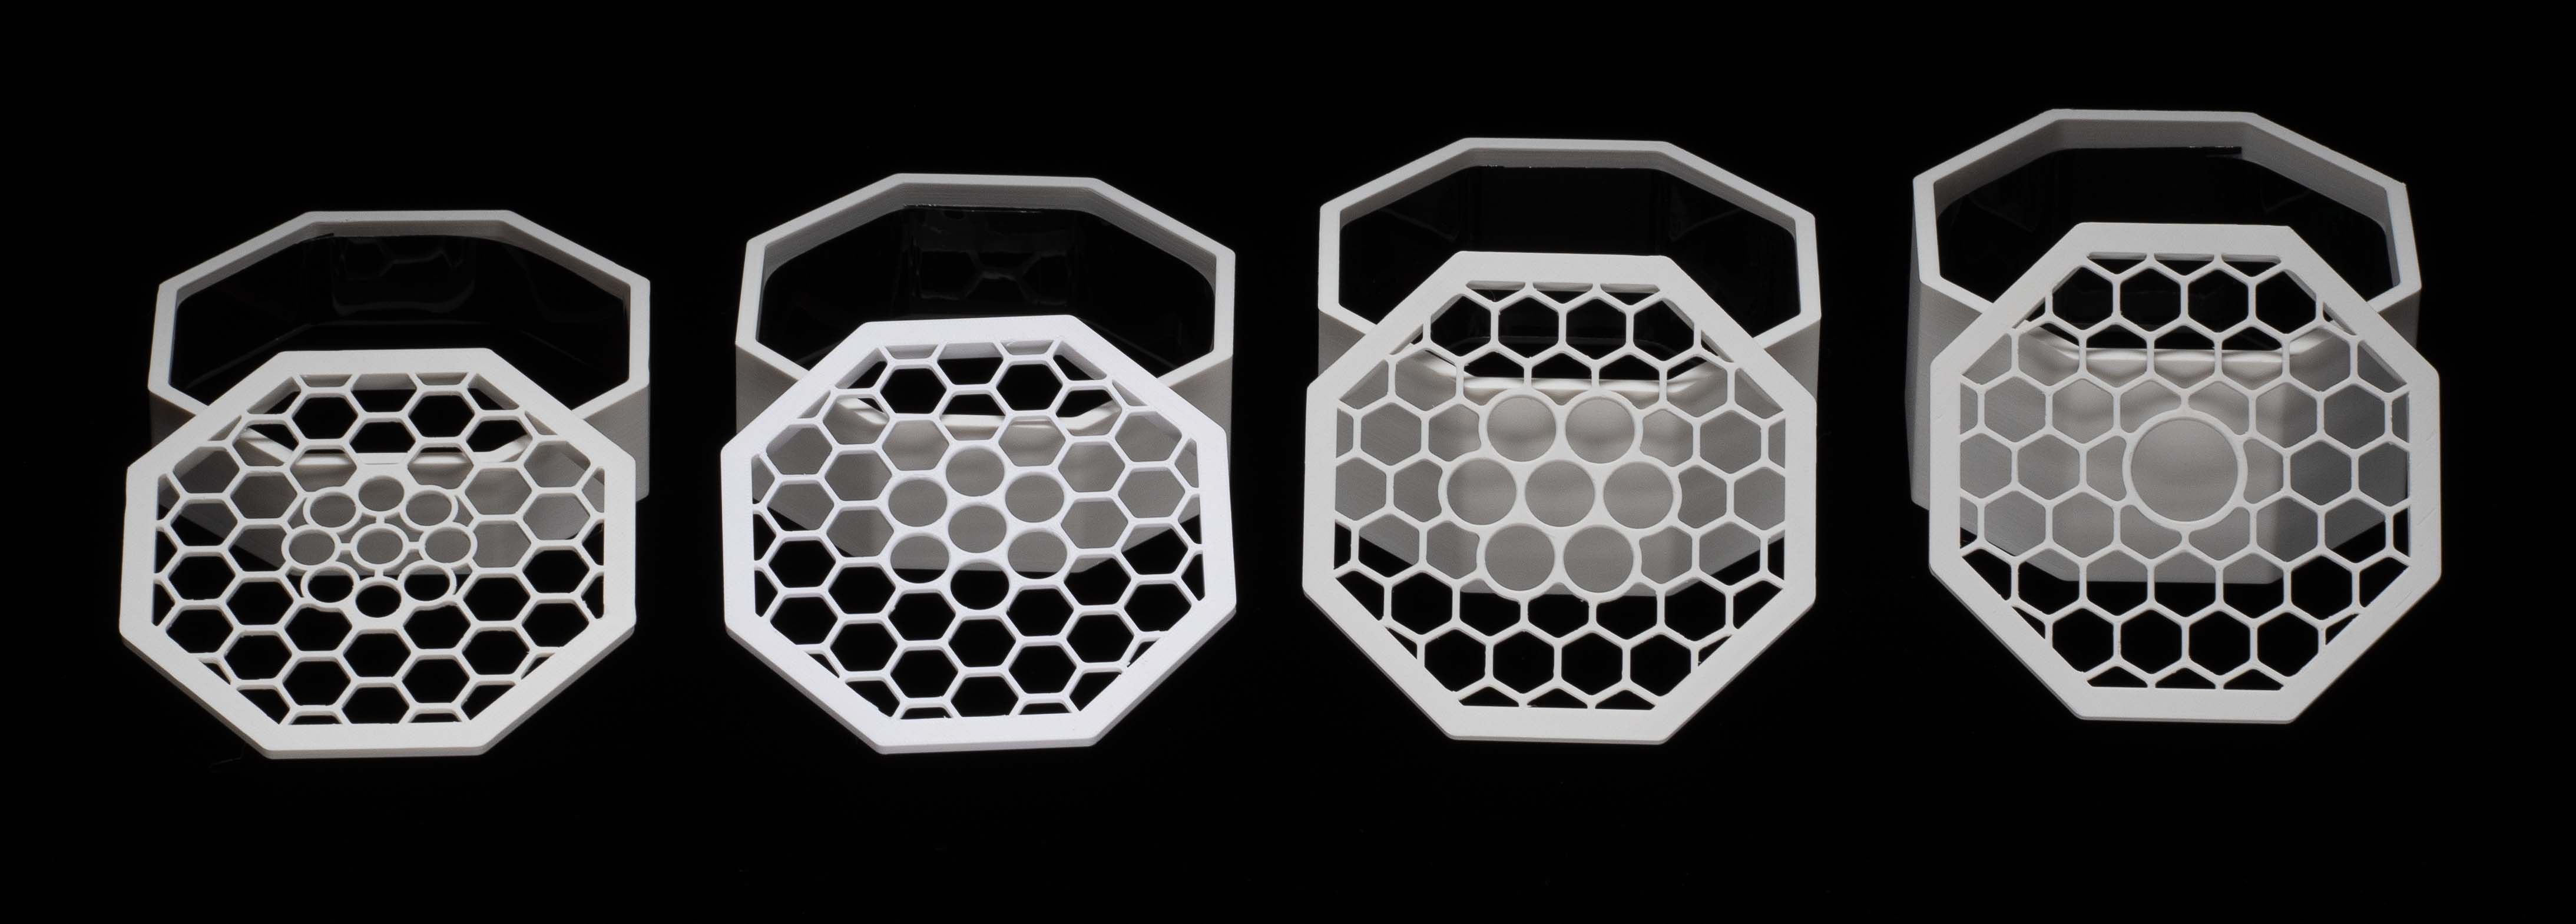
\includegraphics[width=\textwidth]{"./3dp-coverat.jpg"}

The body of the WPR is made up of three main pieces.

\begin{itemize}
    \item Base, containing LEDs, fan, and drive electronics.
    \item Top plate accepting reaction vials.
    \item Walls spacing the top plate at the appropriate distance away from the base.
\end{itemize}

The WPR base is the same for all reactors.
The top plate and wall height can be adjusted depending on the particular vials desired.
Look within the repository in the subdirectory ``photoreactor-tops'' to find existing designs of (wall, top) for a number of different vial sizes.
We encourage you to design your own (wall, top) if none of these suit your application.
Consider adding your new designs to repository so that others may benefit from your design efforts.
In addition to these three main components you should also print a cable-anchor for each of your WPR bases.

TODO: SHARE DETAILS ABOUT CAD SOFTWARE.
TODO: MAKE IT CLEAR THAT STL FILES ARE THE RELEVANT EXCHANGE FILE.
TODO: RECOMMEND STL VIEWER.
TODO: RECOMMEND SLICER.

There are many options for getting your enclosures printed.
TODO: DO WE WANT TO GIVE ANY ADVICE ABOUT MATERIAL CHOICE?
TODO: RECOMMEND SPECIFIC MANUFACTURERS.
Of course, you may wish to print multiple (wall, top) types to be used interchangeably with one base.

Once your parts are done you may need to remove extra bonding material with a razor blade or exacto-knife.
The three pieces of your reactor should fit together snugly and securely.

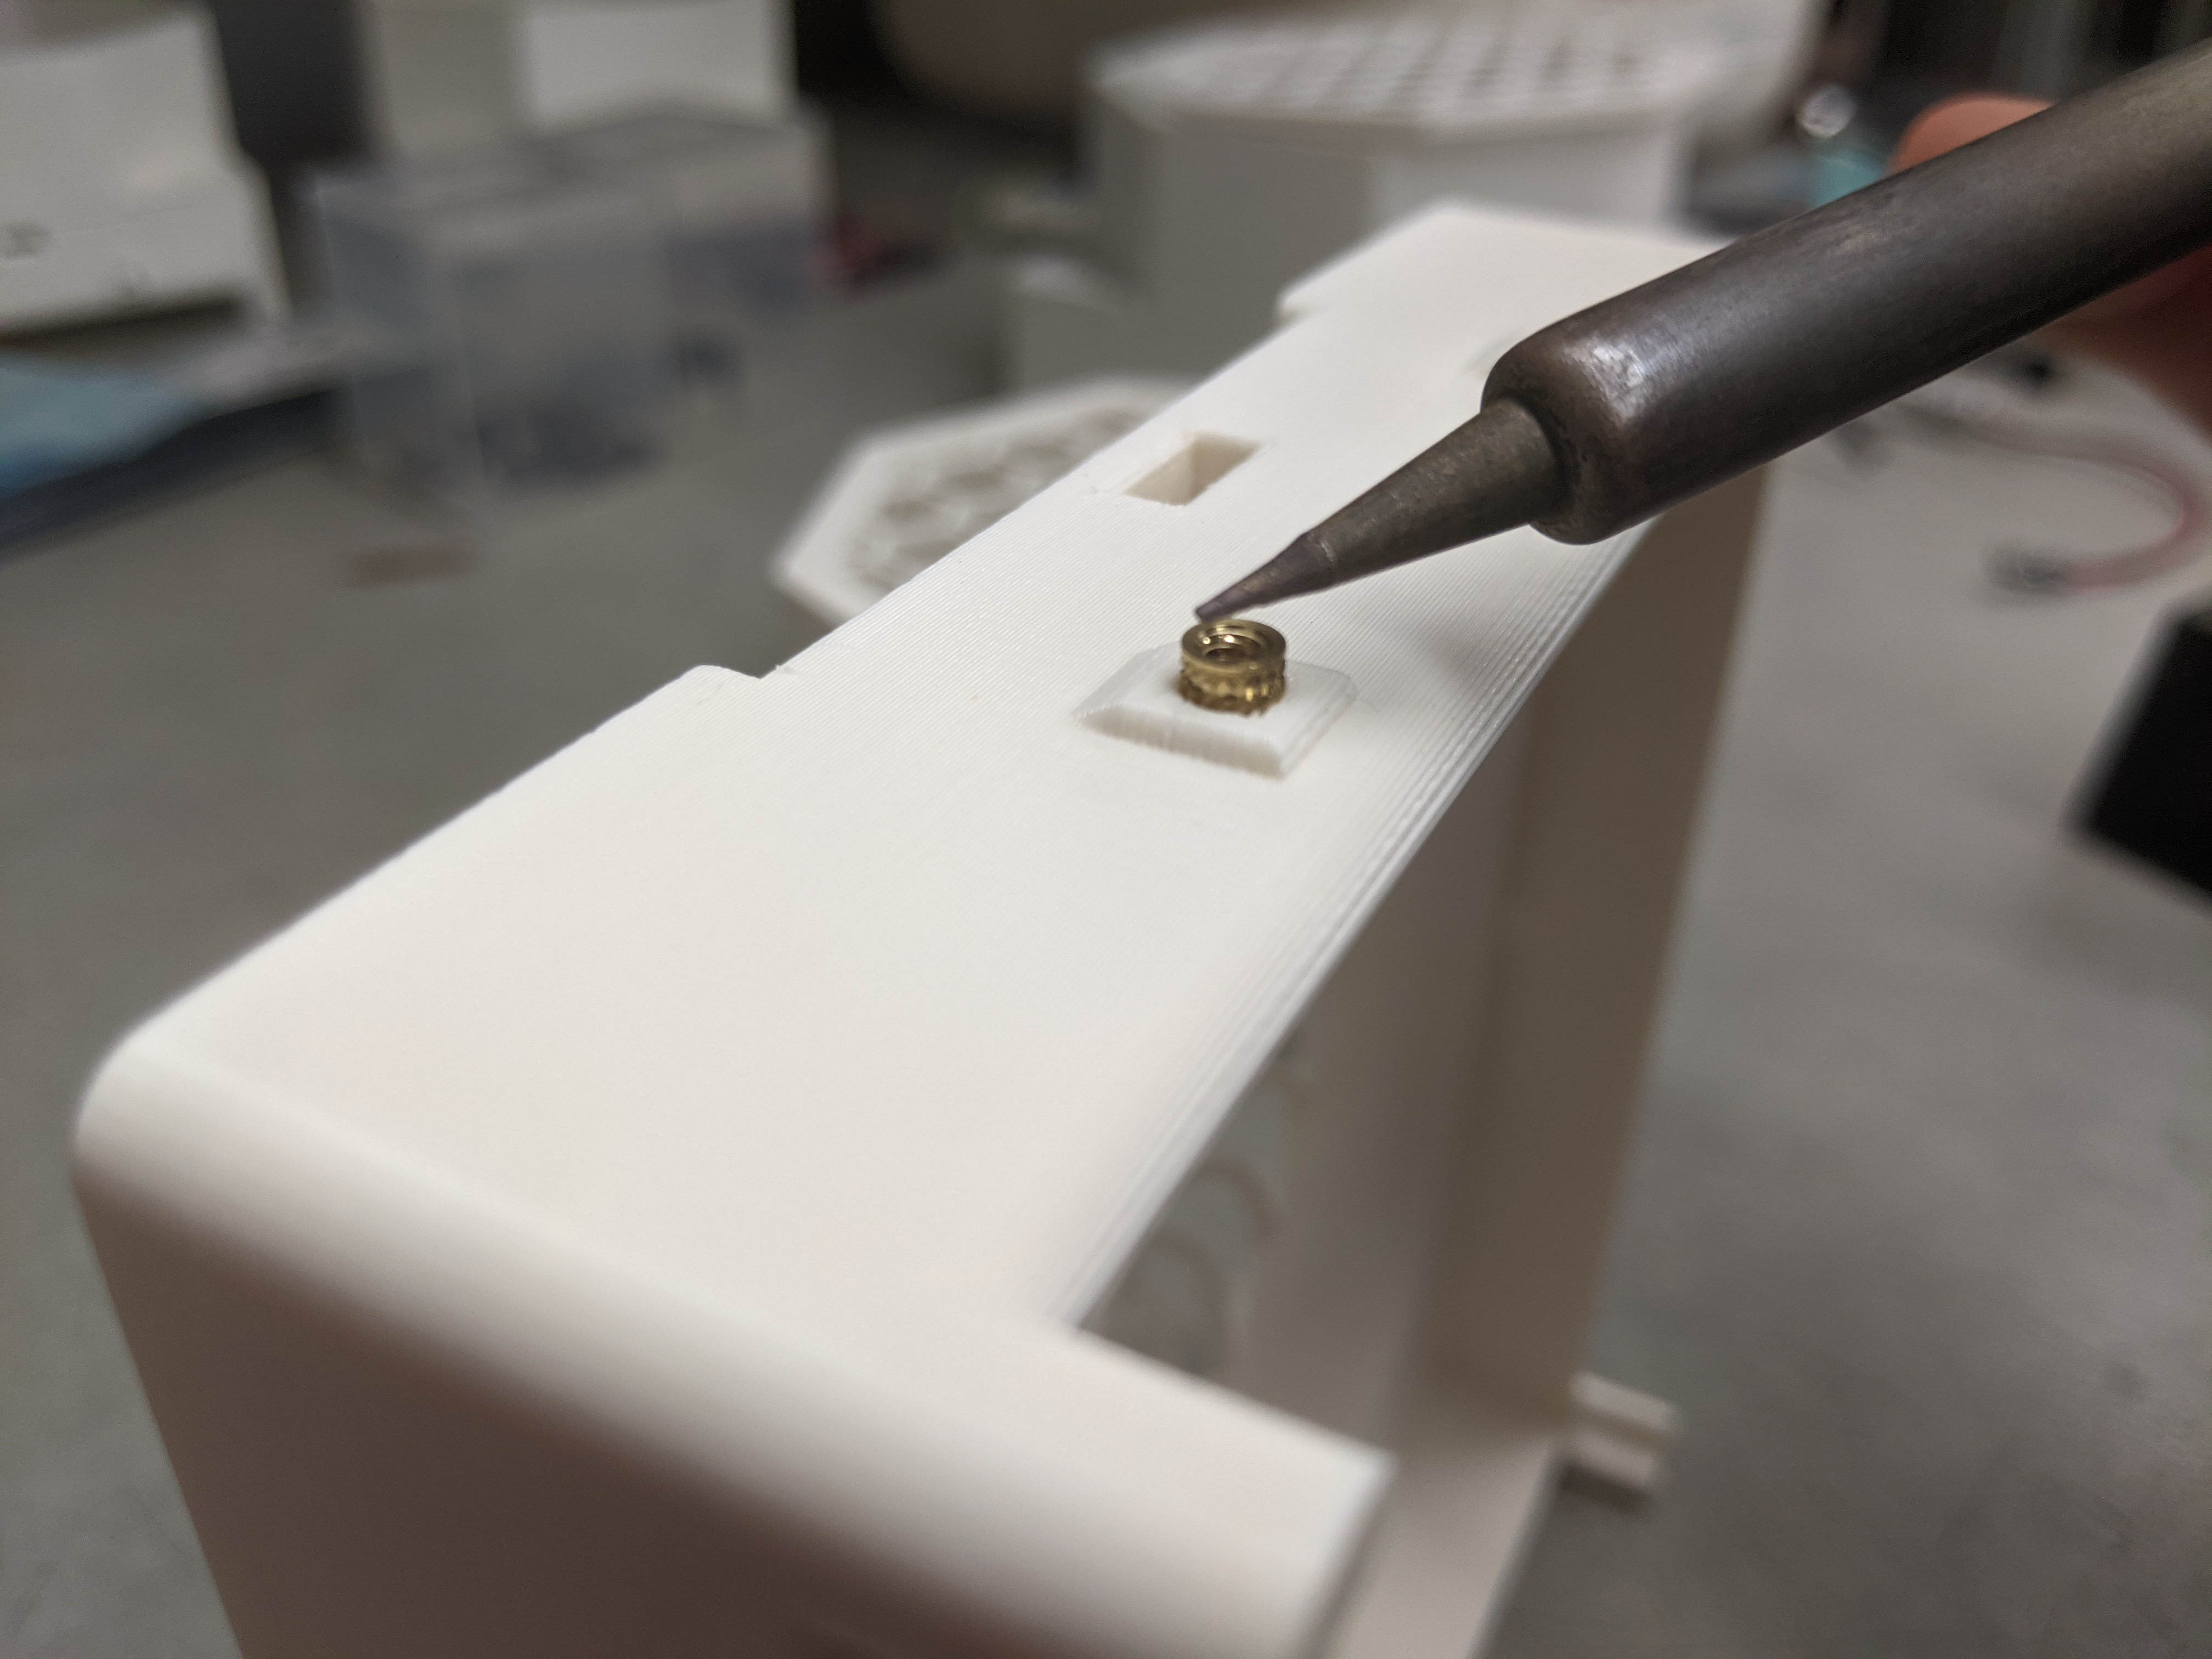
\includegraphics[width=0.5\textwidth]{"./heat-insert.jpg"}

7 heat inserts...

\section{Electronics}

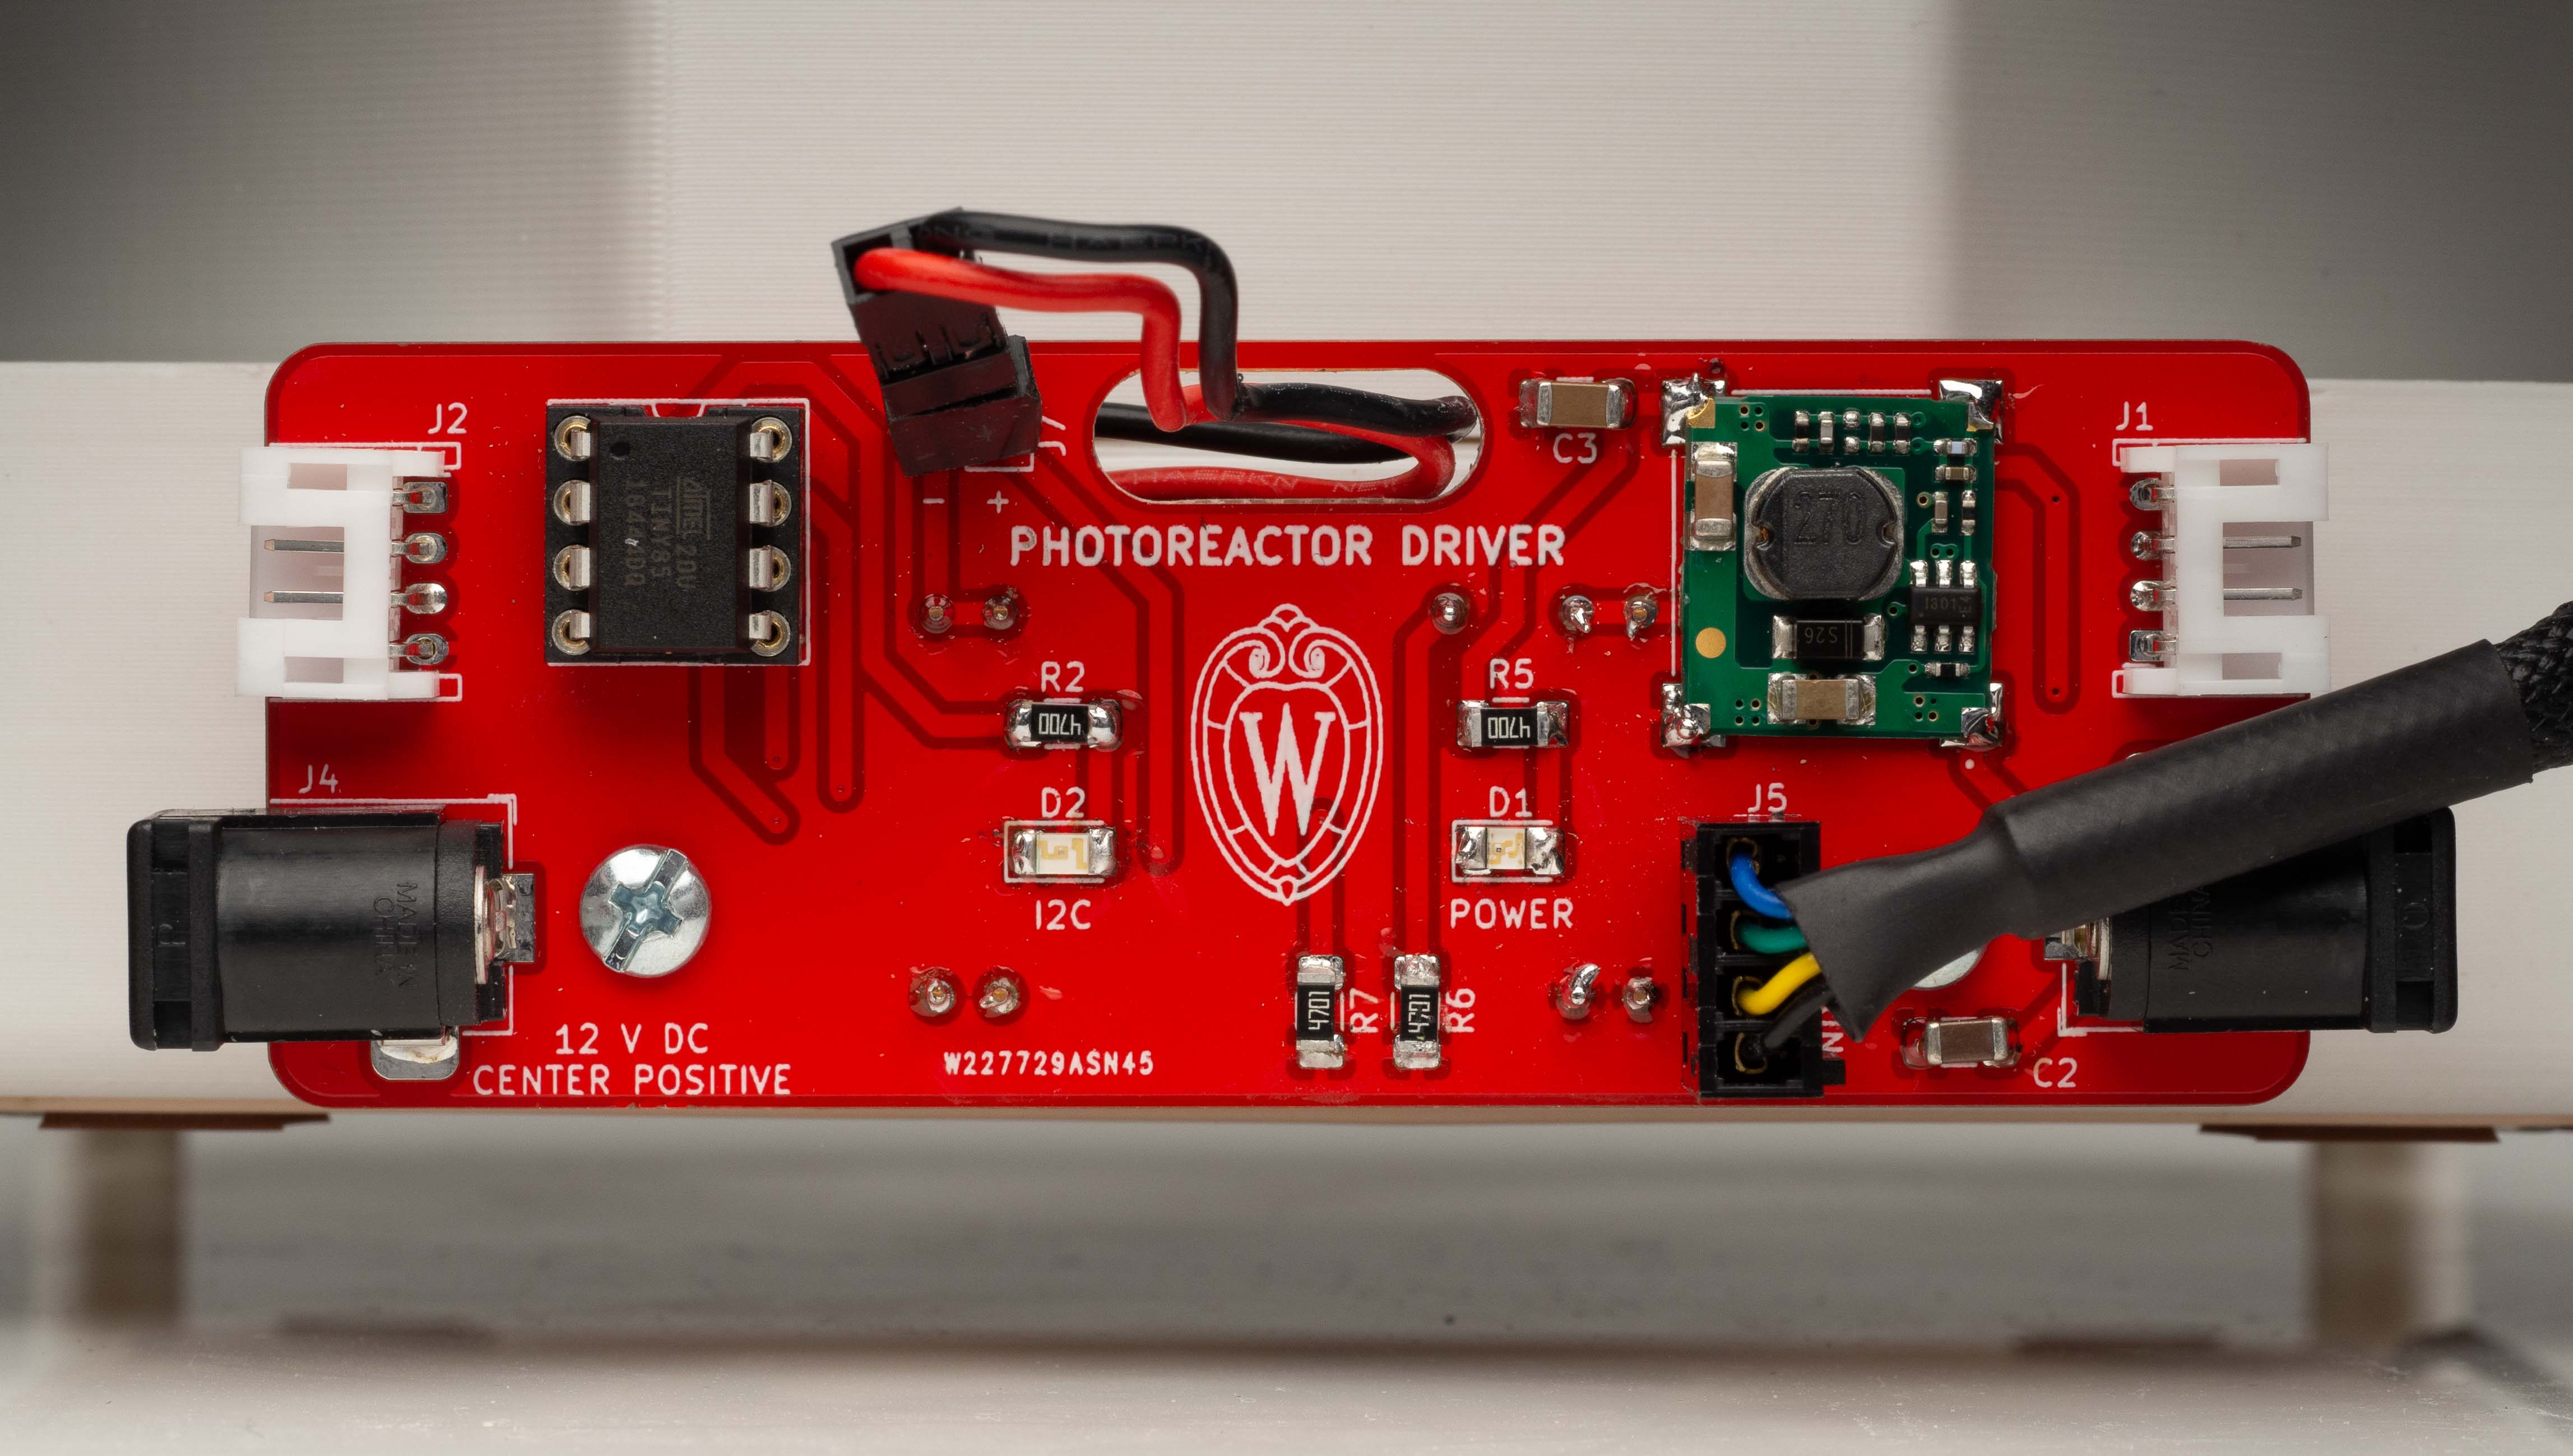
\includegraphics[width=\textwidth]{"./electronics-coverart.jpg"}

The WPR incorporates small circuit boards controlling the incorporated LED and fan.
We refer to these small boards as ``drivers''.
There are two types available: the ``analog-driver'' and ``digital-driver''.
Refer to the associated directories in the online repository for design files for each of these.

The analog-driver circuit is made to be as simple as possible.
The circuit accepts DC 12 V through a barrel jack.
A small knob is used to adjust light intensity.
Fan speed is not adjustable.

The digital-driver circuit is made to be incorporated into an I$^2$C-based digital control system.
In addition to power, these boards have 4-pin connectors to carry the I$^2$C serial data.
More details about this digital control system are in TODO: LINK TO SECTION.

\clearpage
\subsection{Analog}

\begin{center}
  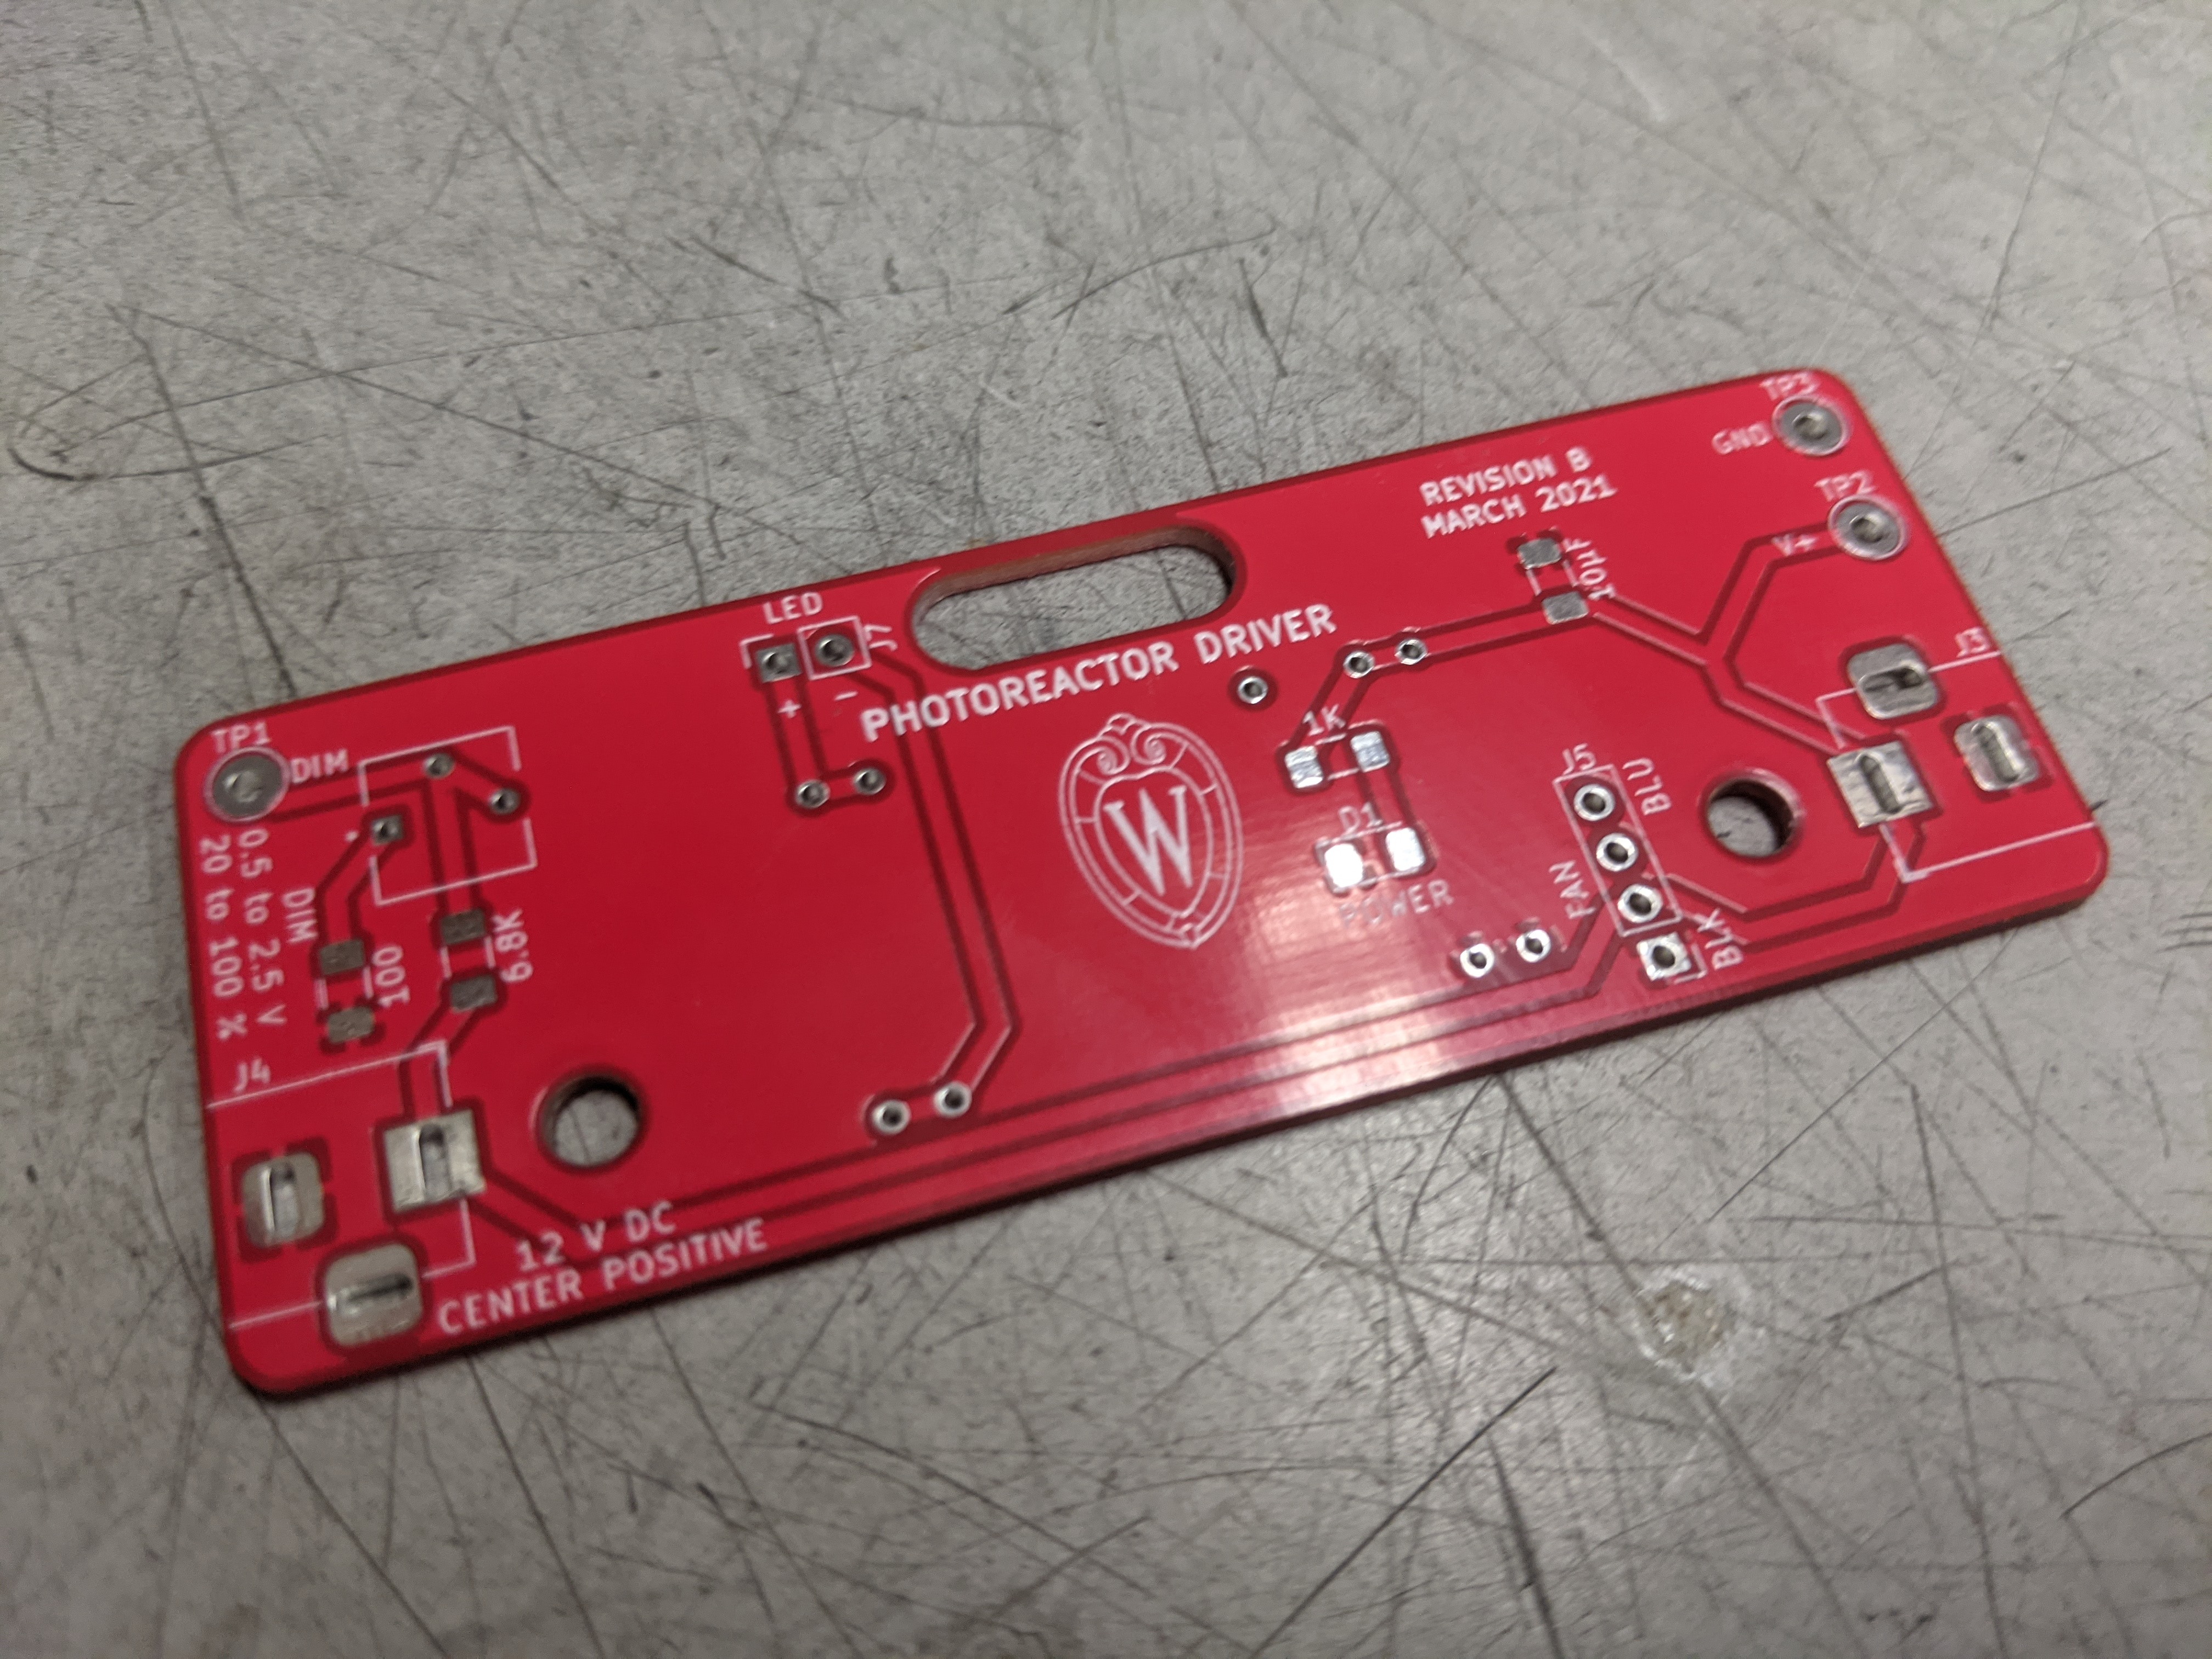
\includegraphics[width=\textwidth/2]{"./bare-pcb.jpg"}
\end{center}

\begin{center}
  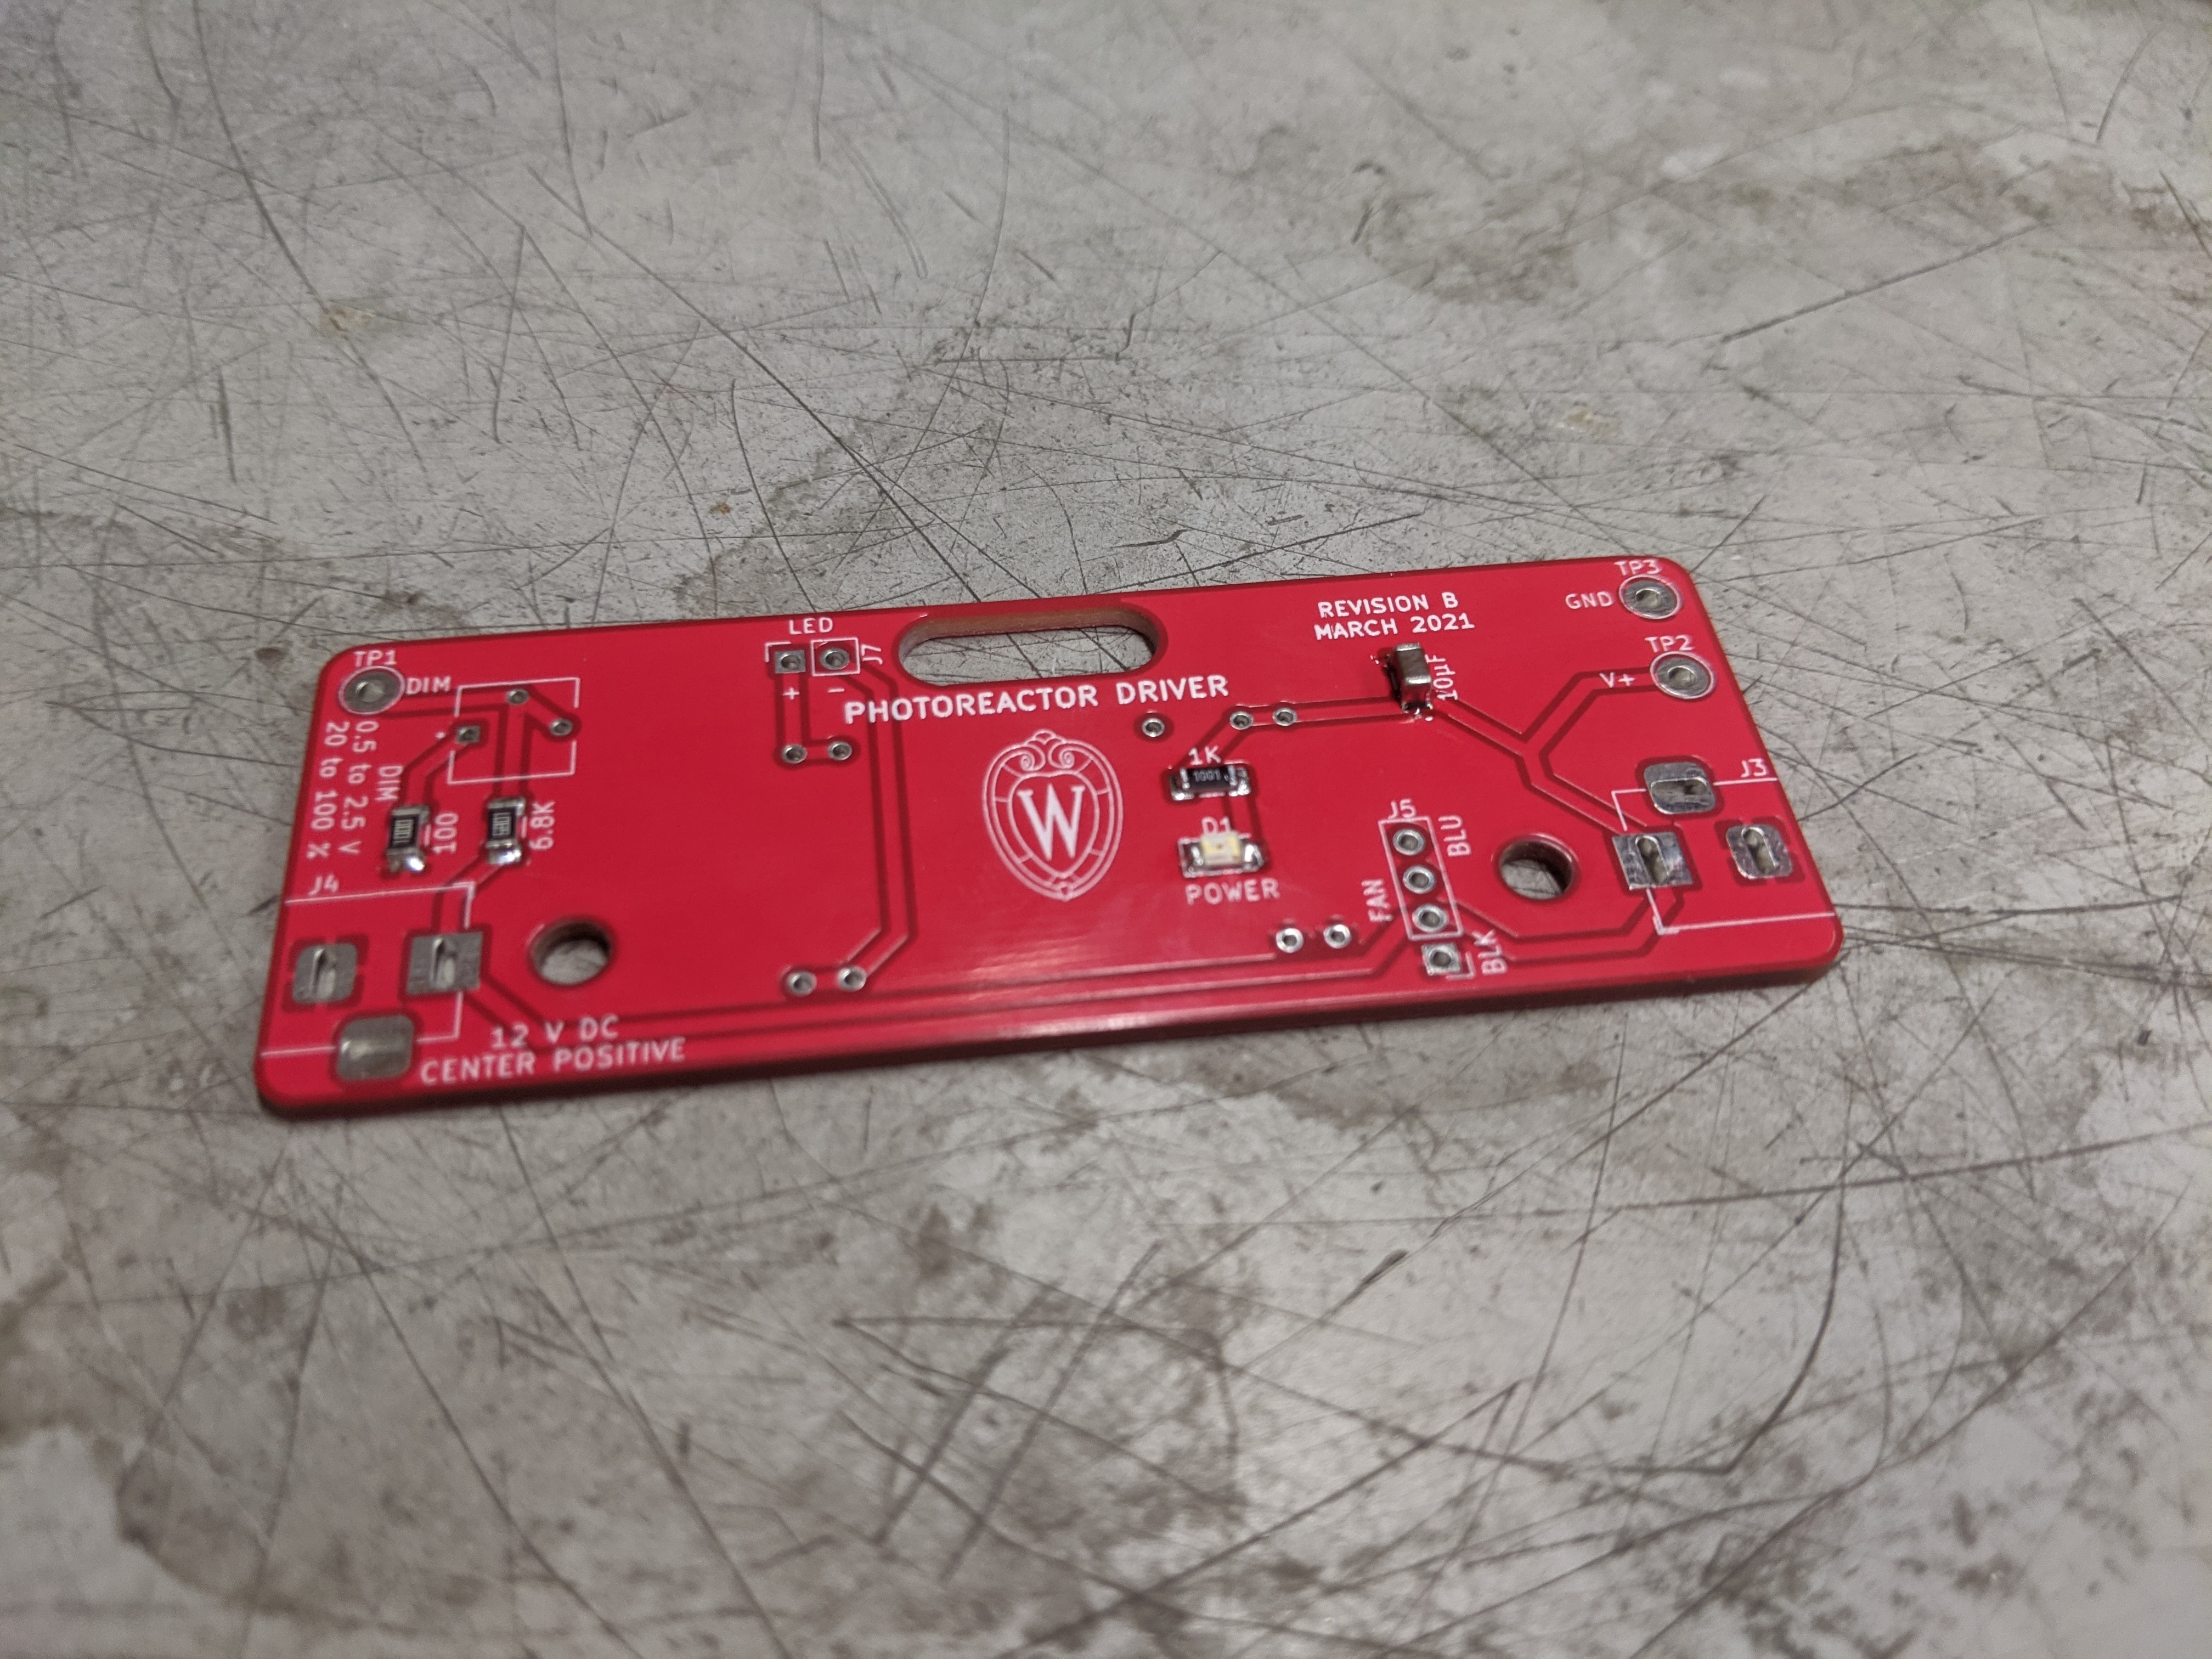
\includegraphics[width=\textwidth/2]{"./surface-mount.jpg"}
\end{center}

Recommend thin solder, e.g. 0.015''.
Small green line on LED towards ground (left).

\begin{center}
  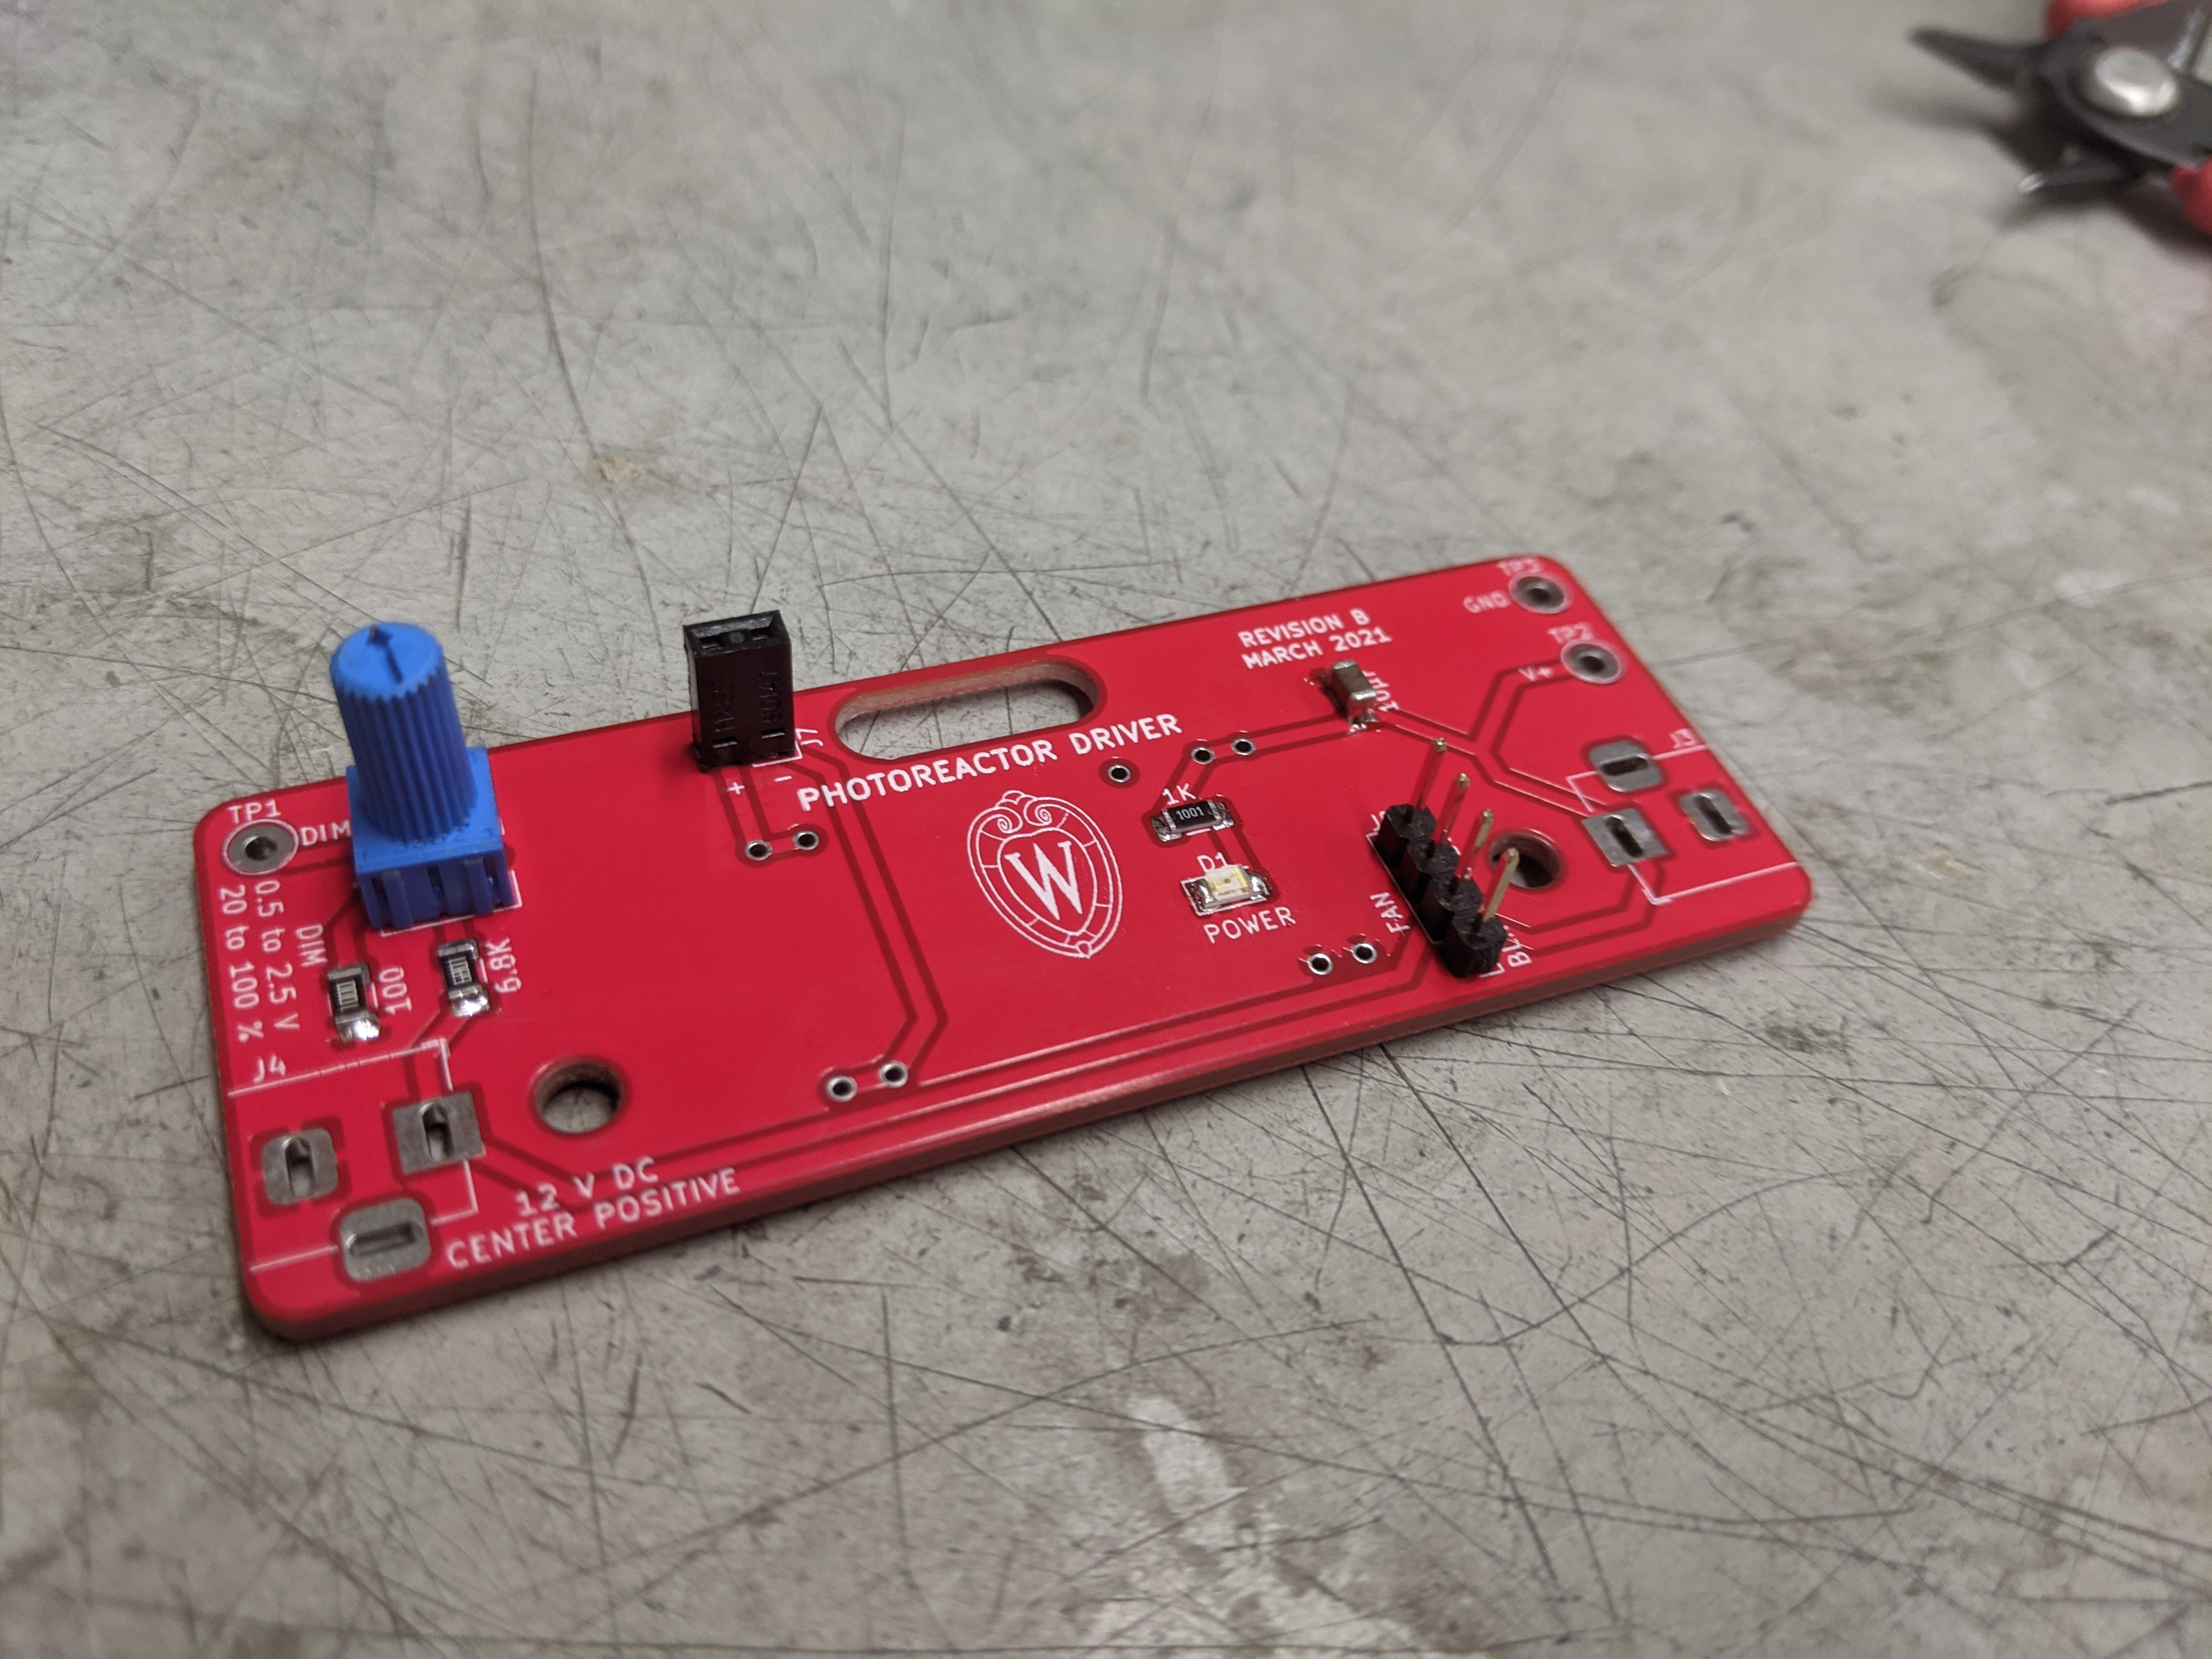
\includegraphics[width=\textwidth/2]{"./connectors.jpg"}
\end{center}

Recommend standard solder, e.g. 0.031''.

\begin{center}
  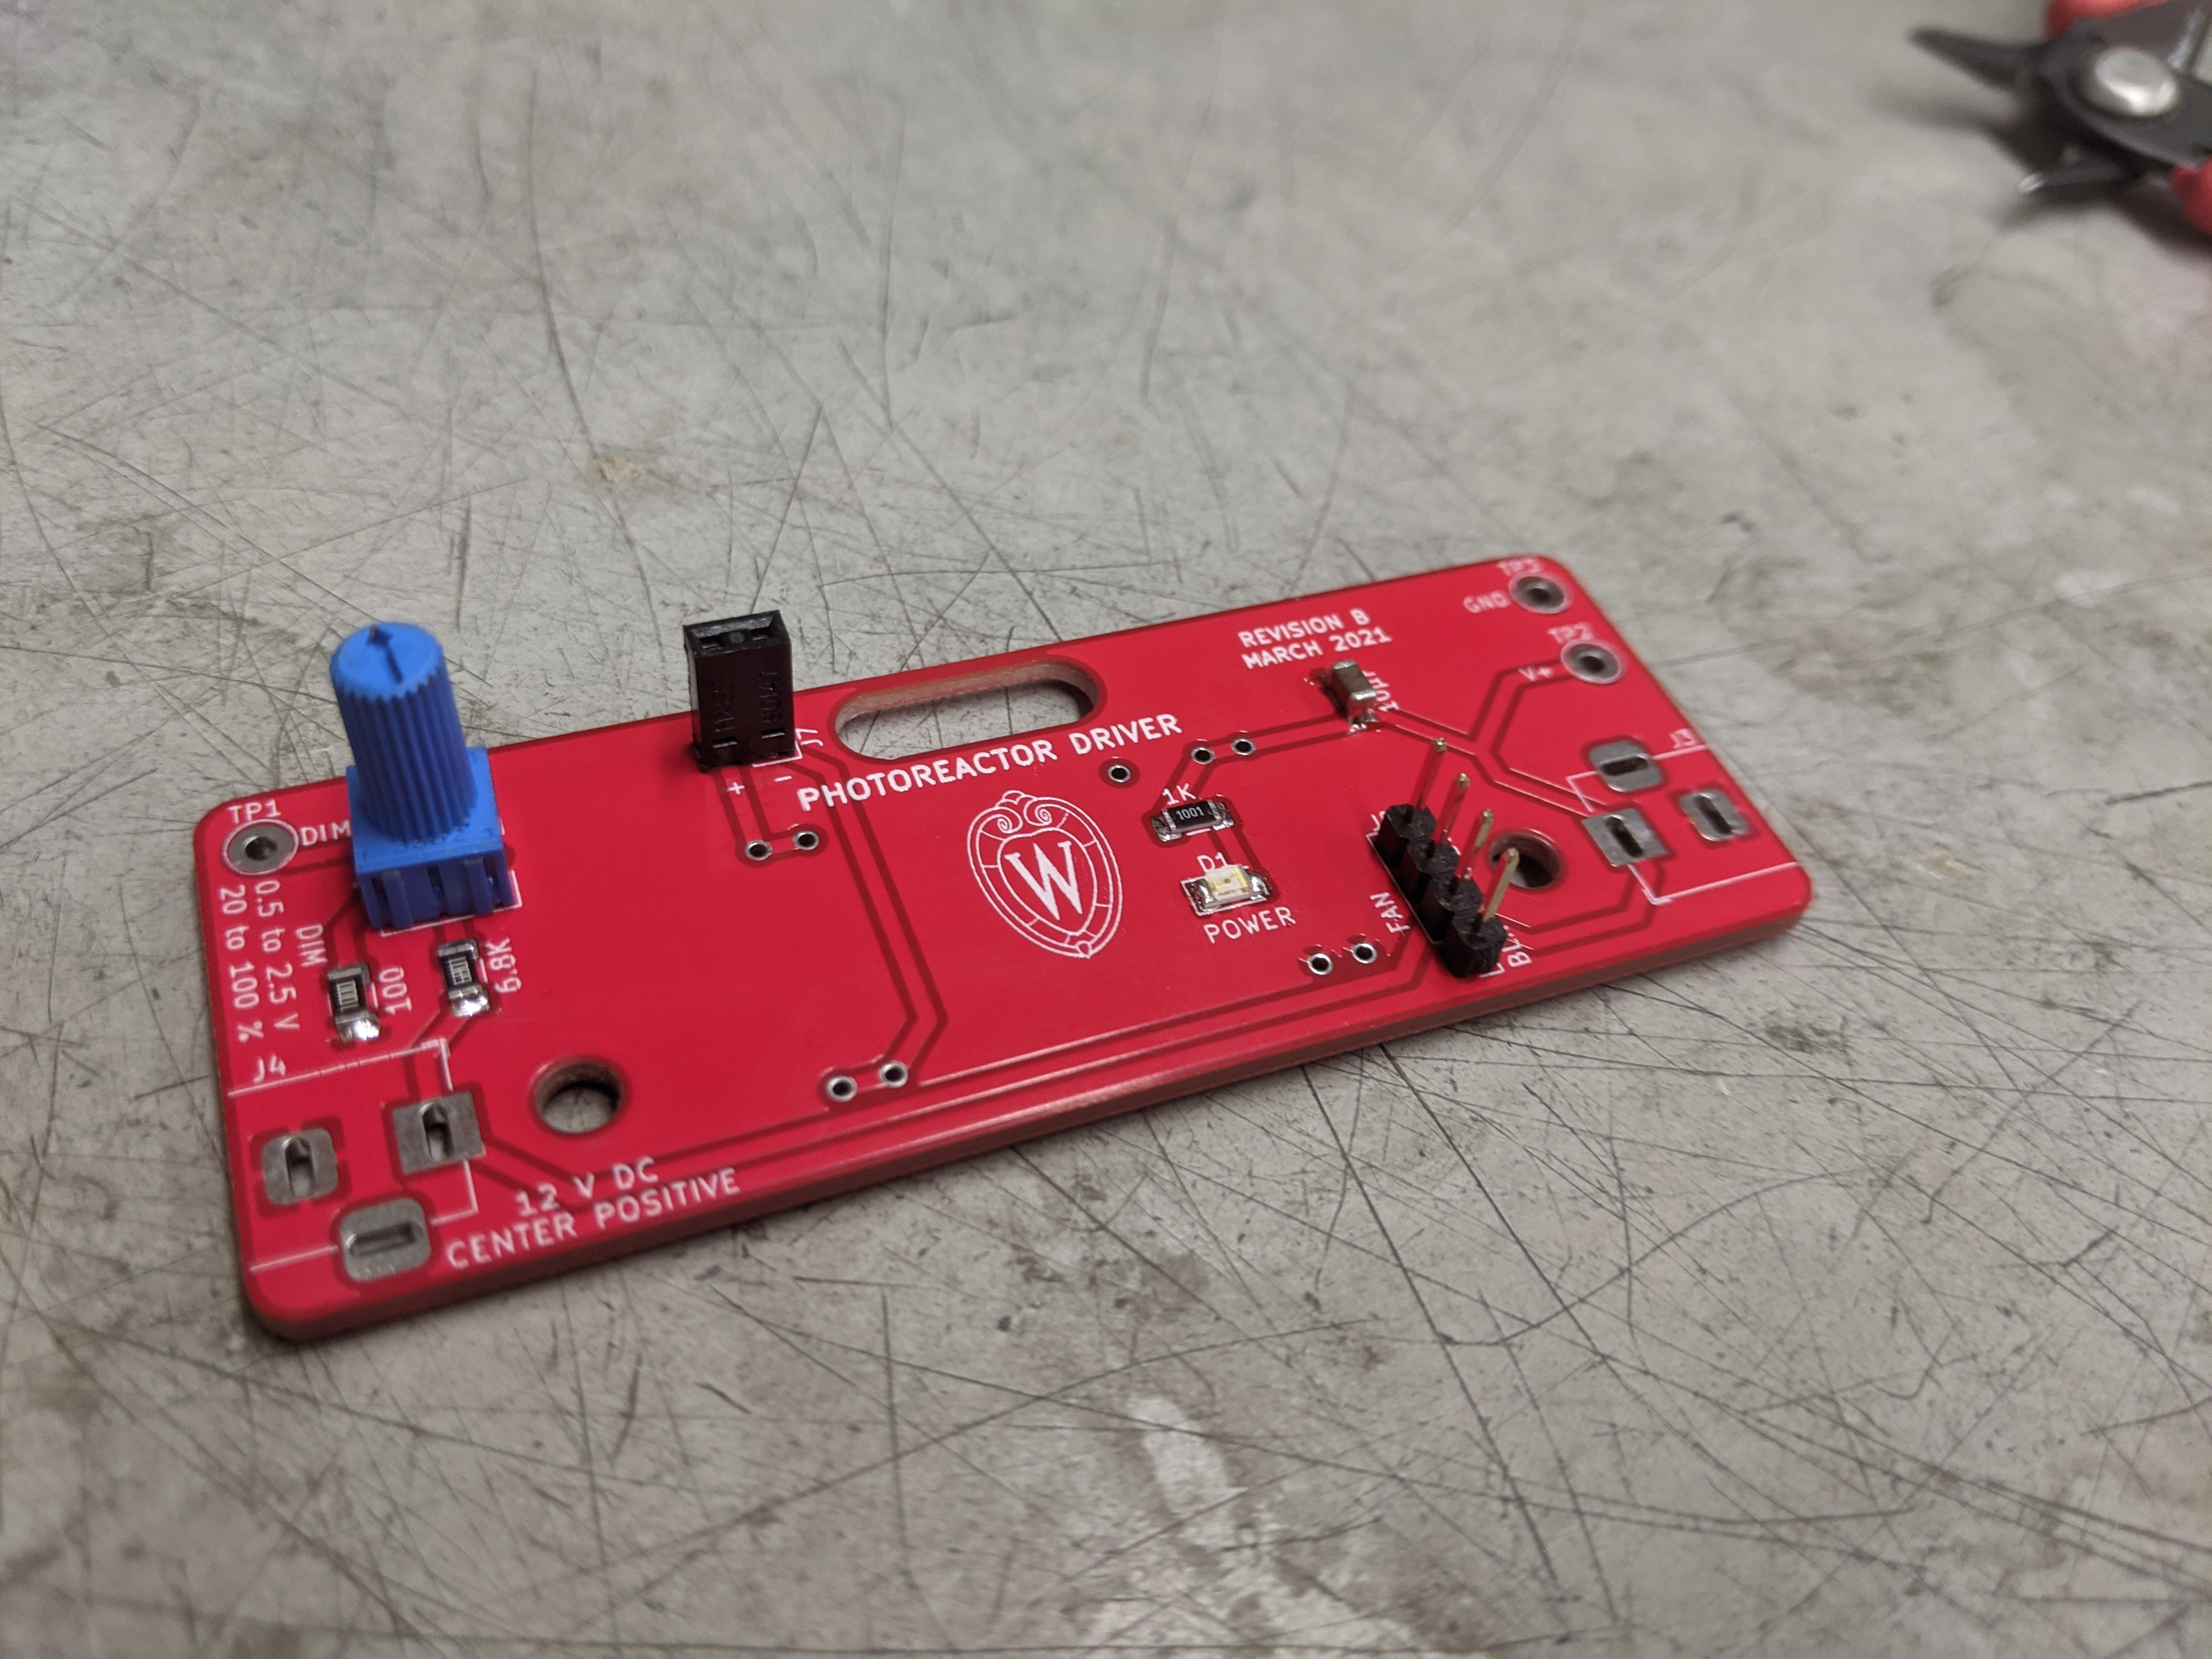
\includegraphics[width=\textwidth/2]{"./connectors.jpg"}
\end{center}

\begin{center}
  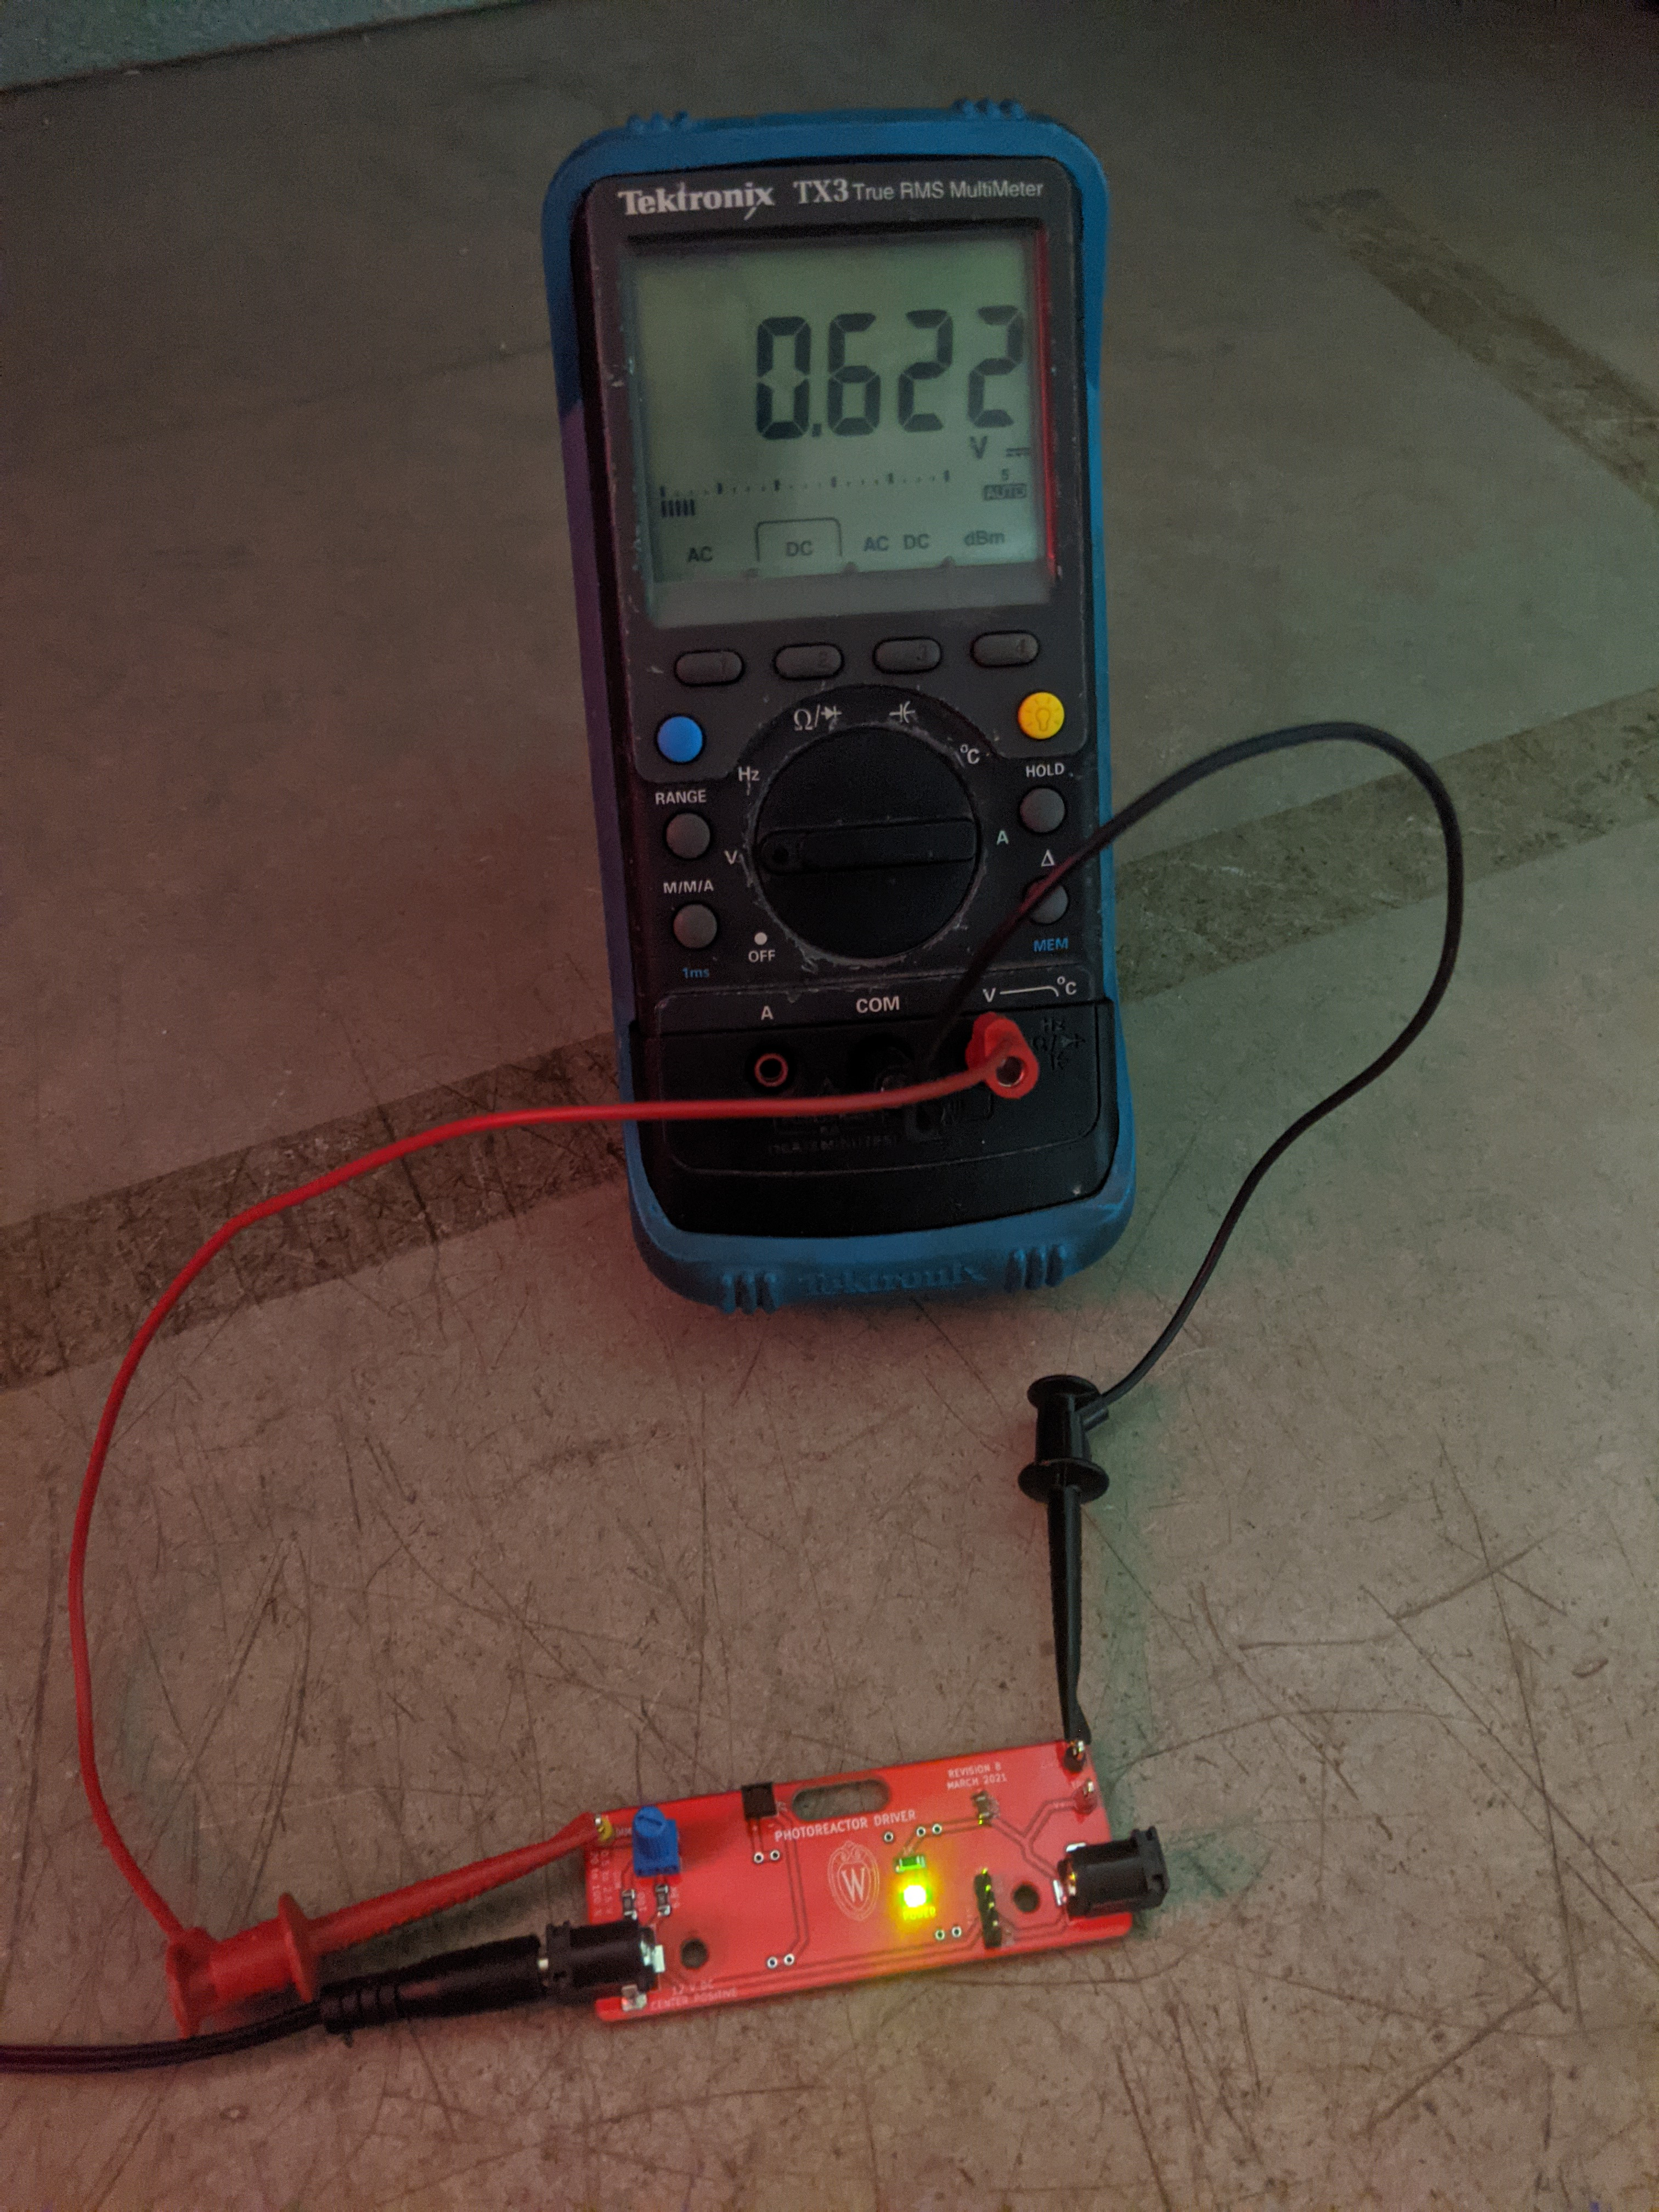
\includegraphics[width=\textwidth/2]{"./barrels-tested.jpg"}
\end{center}

\begin{center}
  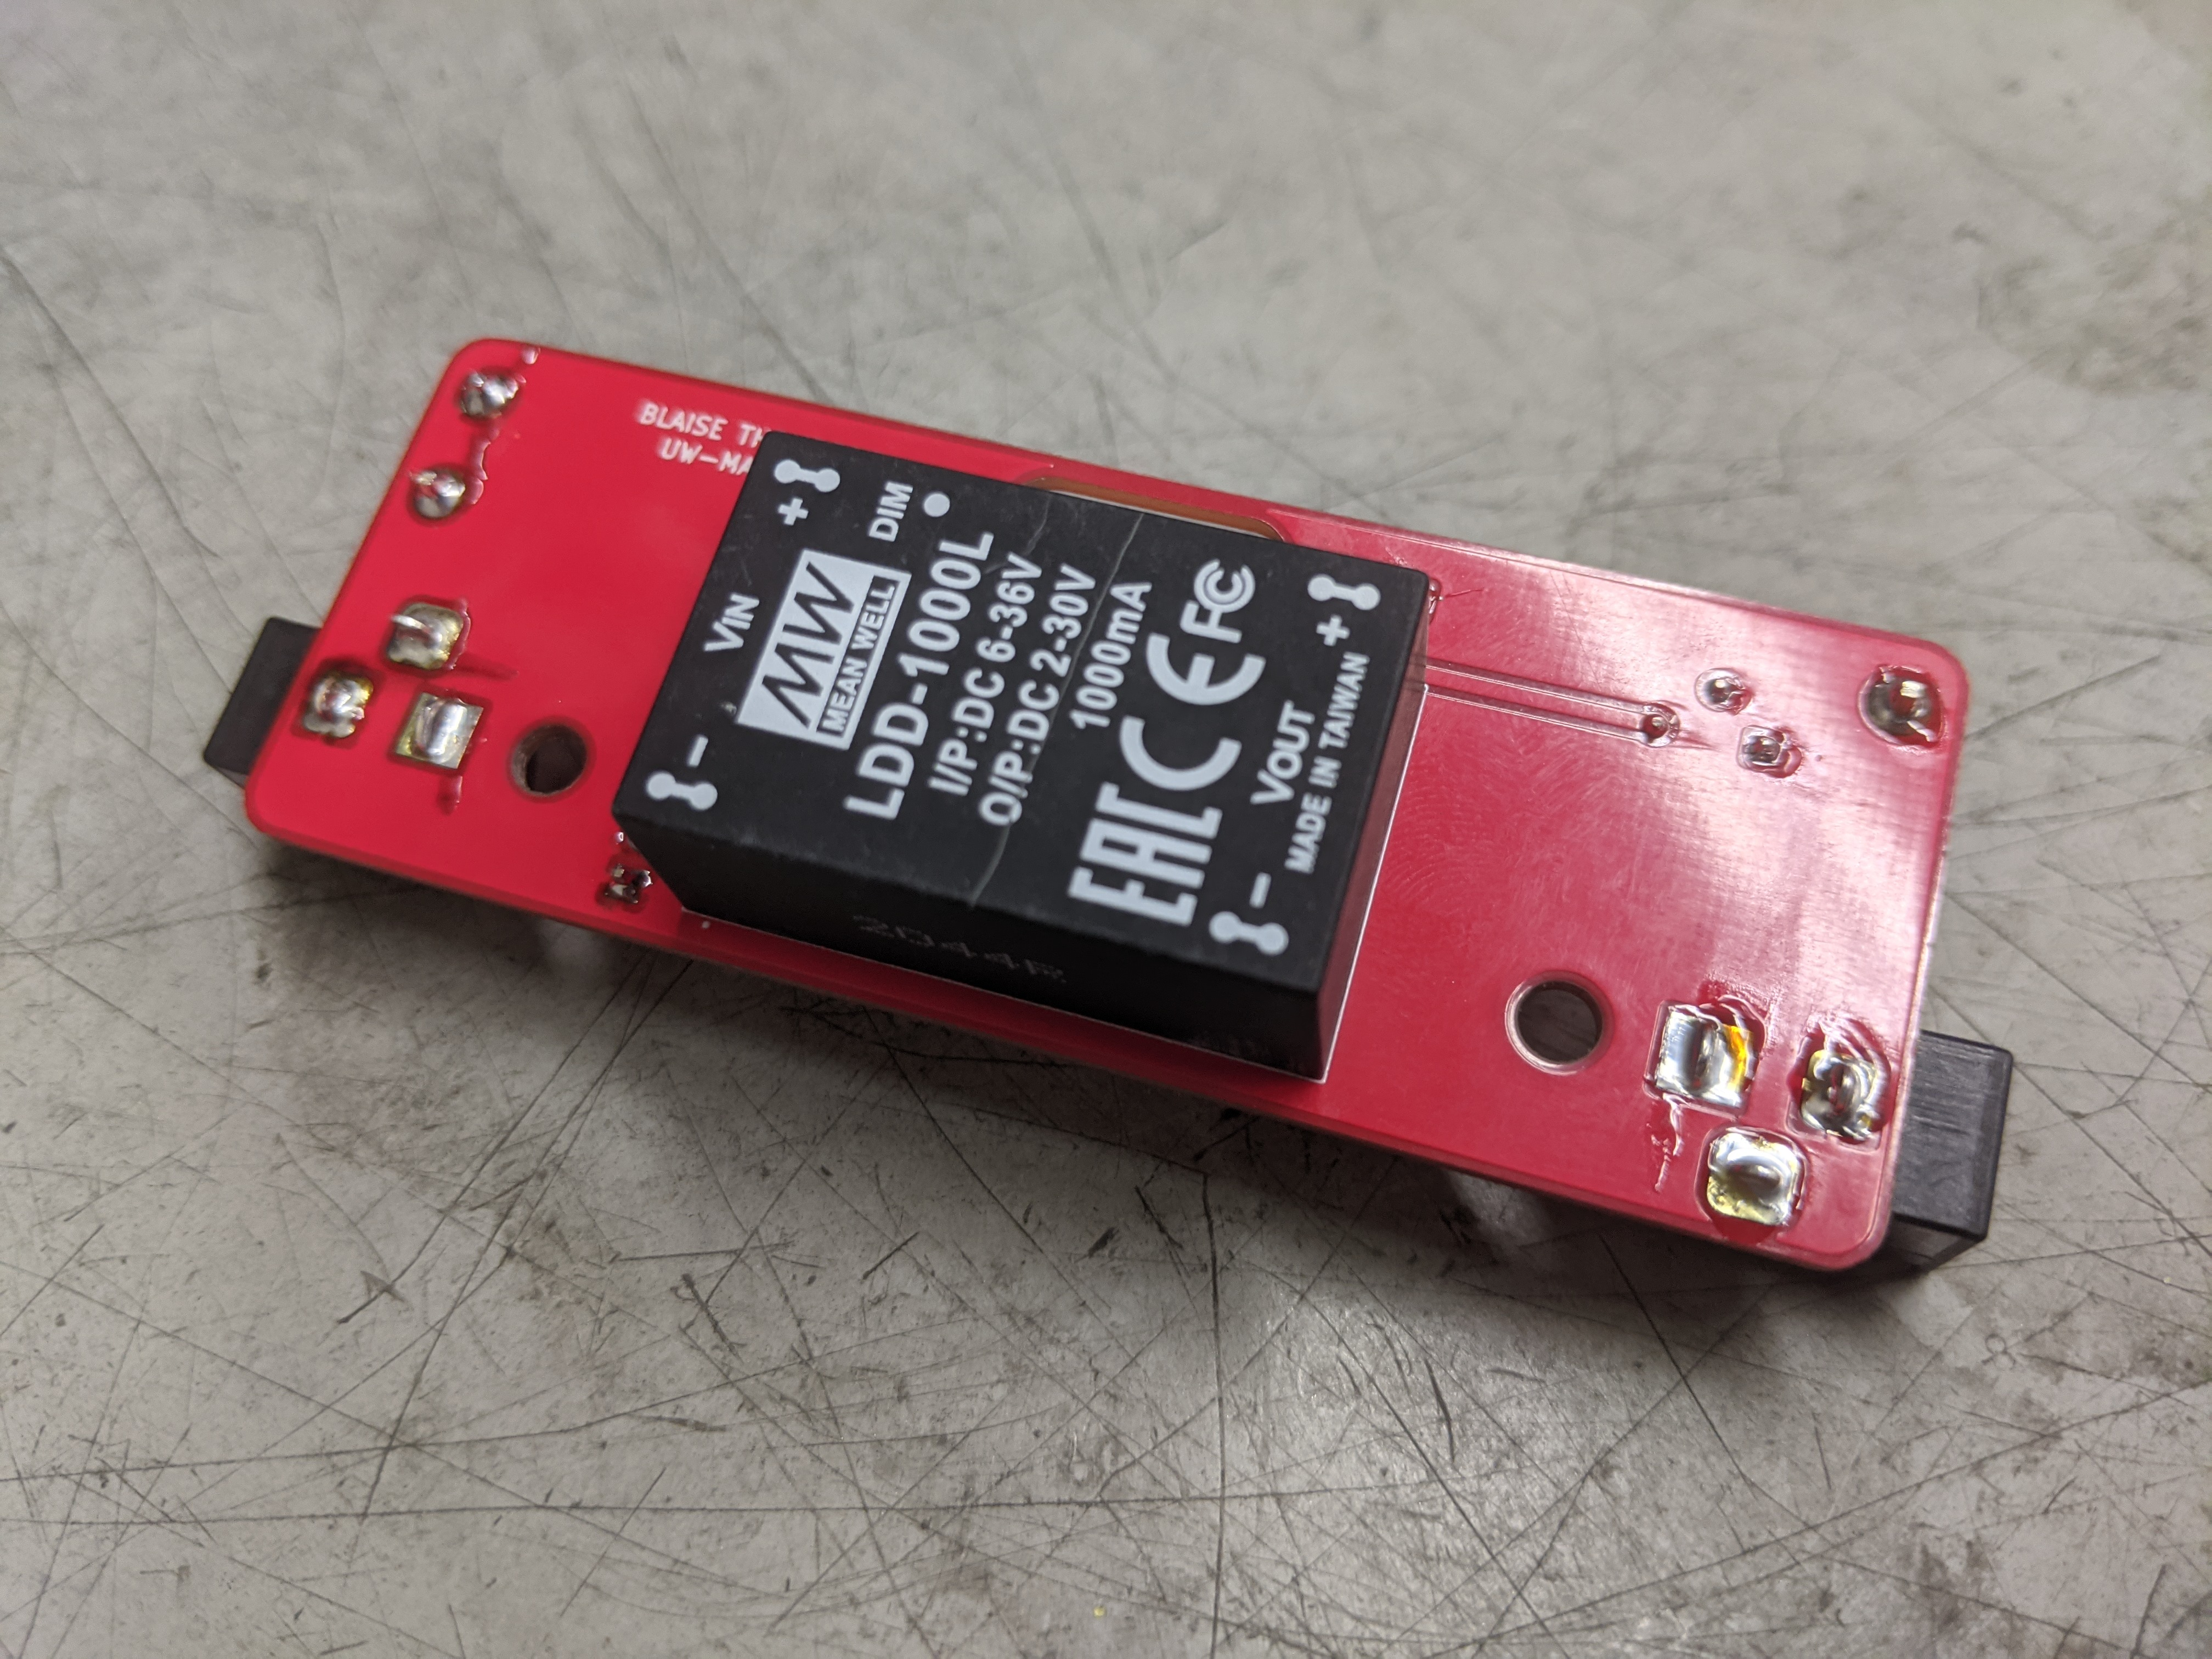
\includegraphics[width=\textwidth/2]{"./pcb-driver.jpg"}
\end{center}

150 mA to 3 V

TODO: ADD DRIVER

\includepdf[landscape=true]{"../analog-driver/driver.pdf"}

\subsection{Digital}

TODO: document I2C connection choice.
Consistent with Adafruit, Sparkfun, Seeed...

\subsubsection{Driver}

\includepdf[landscape=true]{"../digital-driver/driver.pdf"}

\subsubsection{Controller}

\section{Assembly}

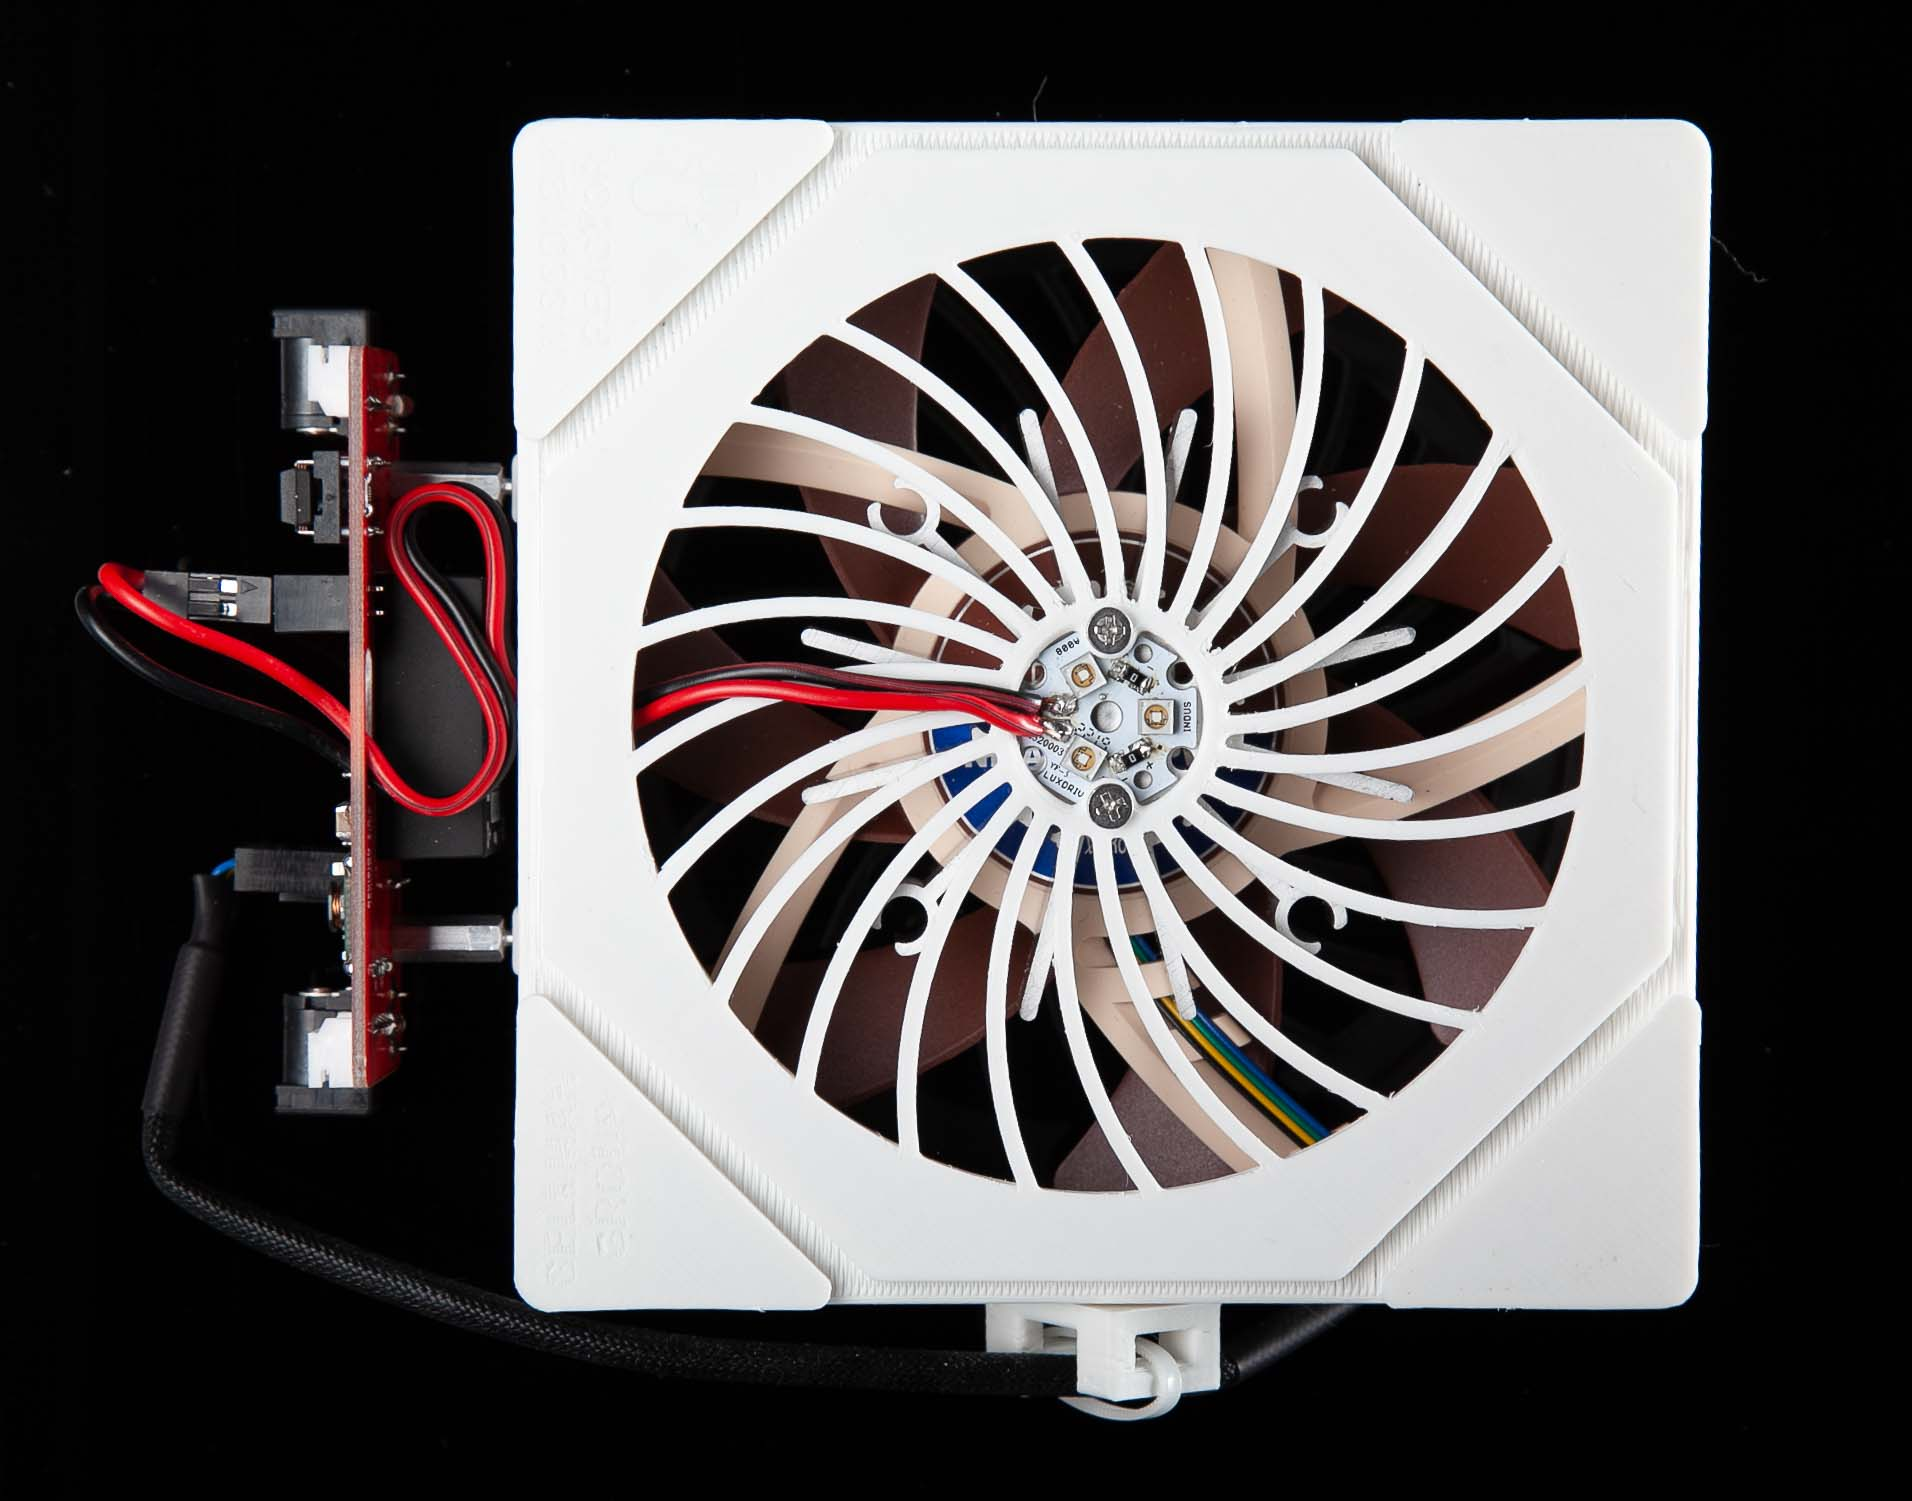
\includegraphics[width=\textwidth]{"./assembly-coverart.jpg"}

0.5'' standoff: RAF 4505-440-AL

\subsection{Base}

TODO: ASSEMBLE LED
In this case LED Supply 07007-PL000-F
May be a challenge---heat sinking will fight you
Add lead-based solder to make easier

TODO: LED PCB part number

TODO: LED PINS SOLUTION

TODO: heatsink part number

\begin{center}
  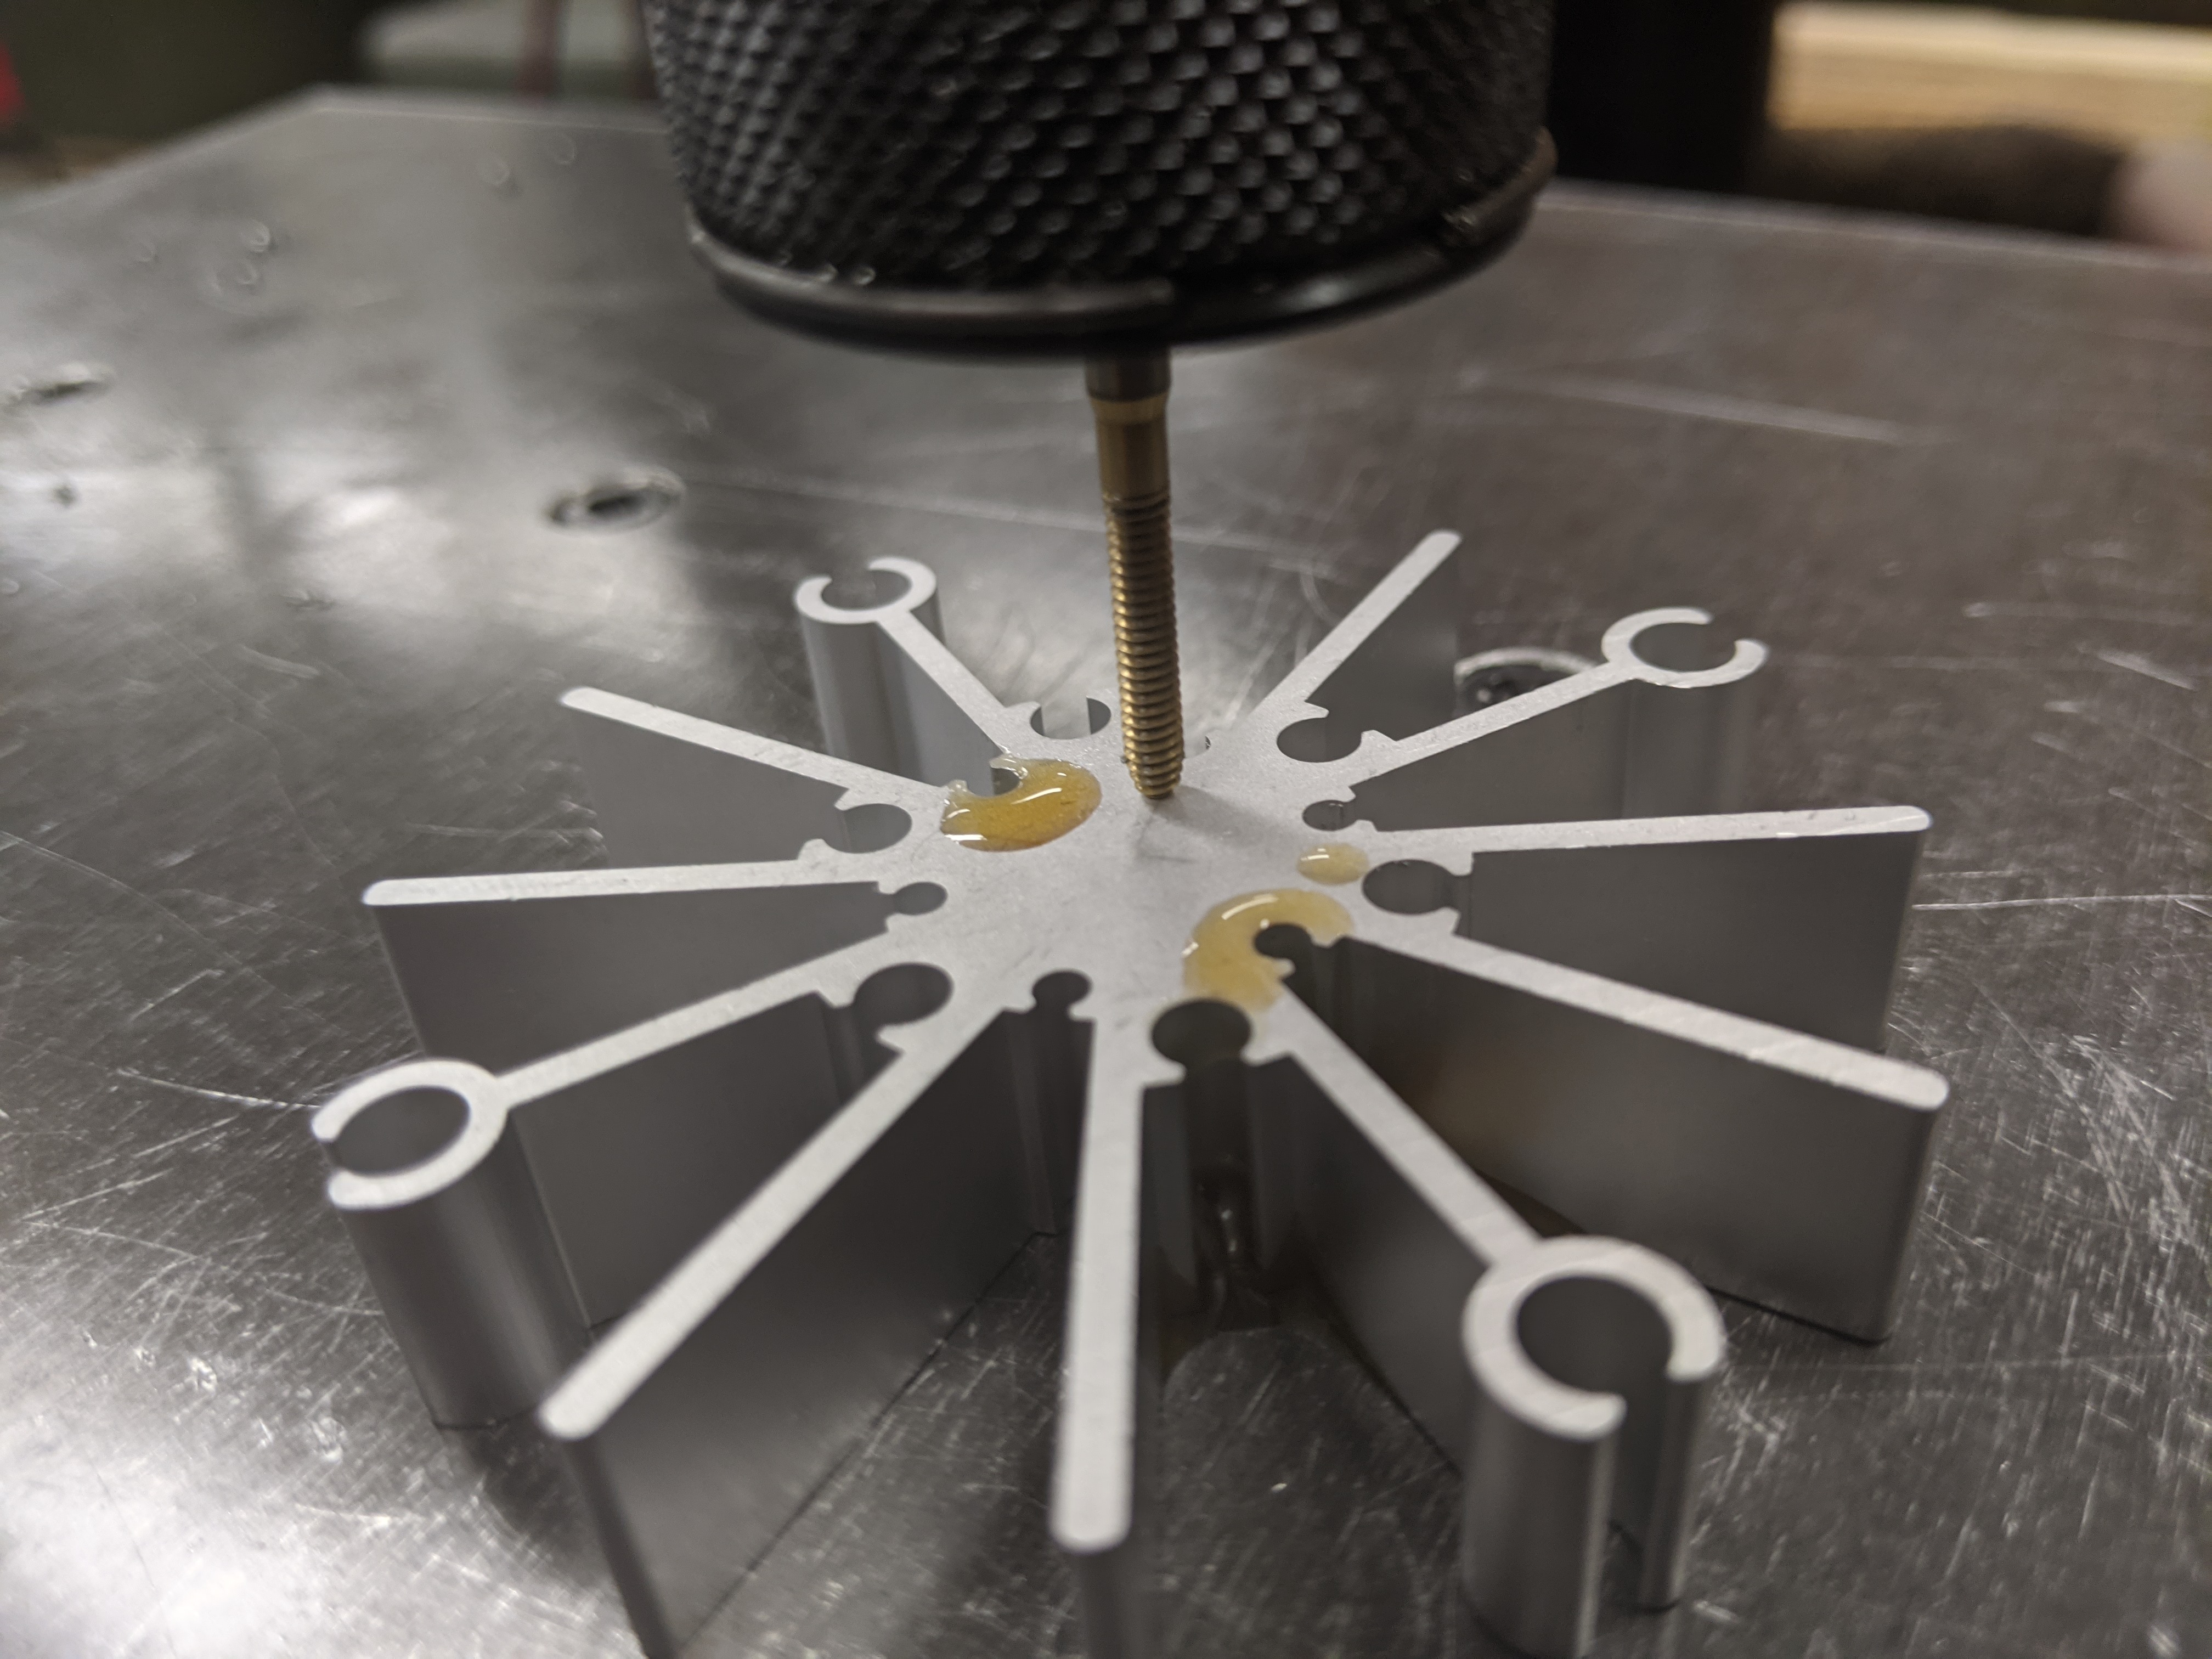
\includegraphics[width=\textwidth/2]{"./tap-heatsink.jpg"}
\end{center}

Tap the heatsink.
We used thread-forming tap: OSG 1400105300.

TODO: heatsink compoud

Install with wires facing towards printed hole

Use 4-40 1/4''.   Fastenal 0146455

TODO: MOUNT FAN

Noctua NF-A12x15 PWM

pins:
blue: PWM (5 V)
yellow: +12 V
black: ground

Use 4-40 3/4'' into captured nuts

TODO: cable tie

\subsubsection{Reflector}

\begin{center}
  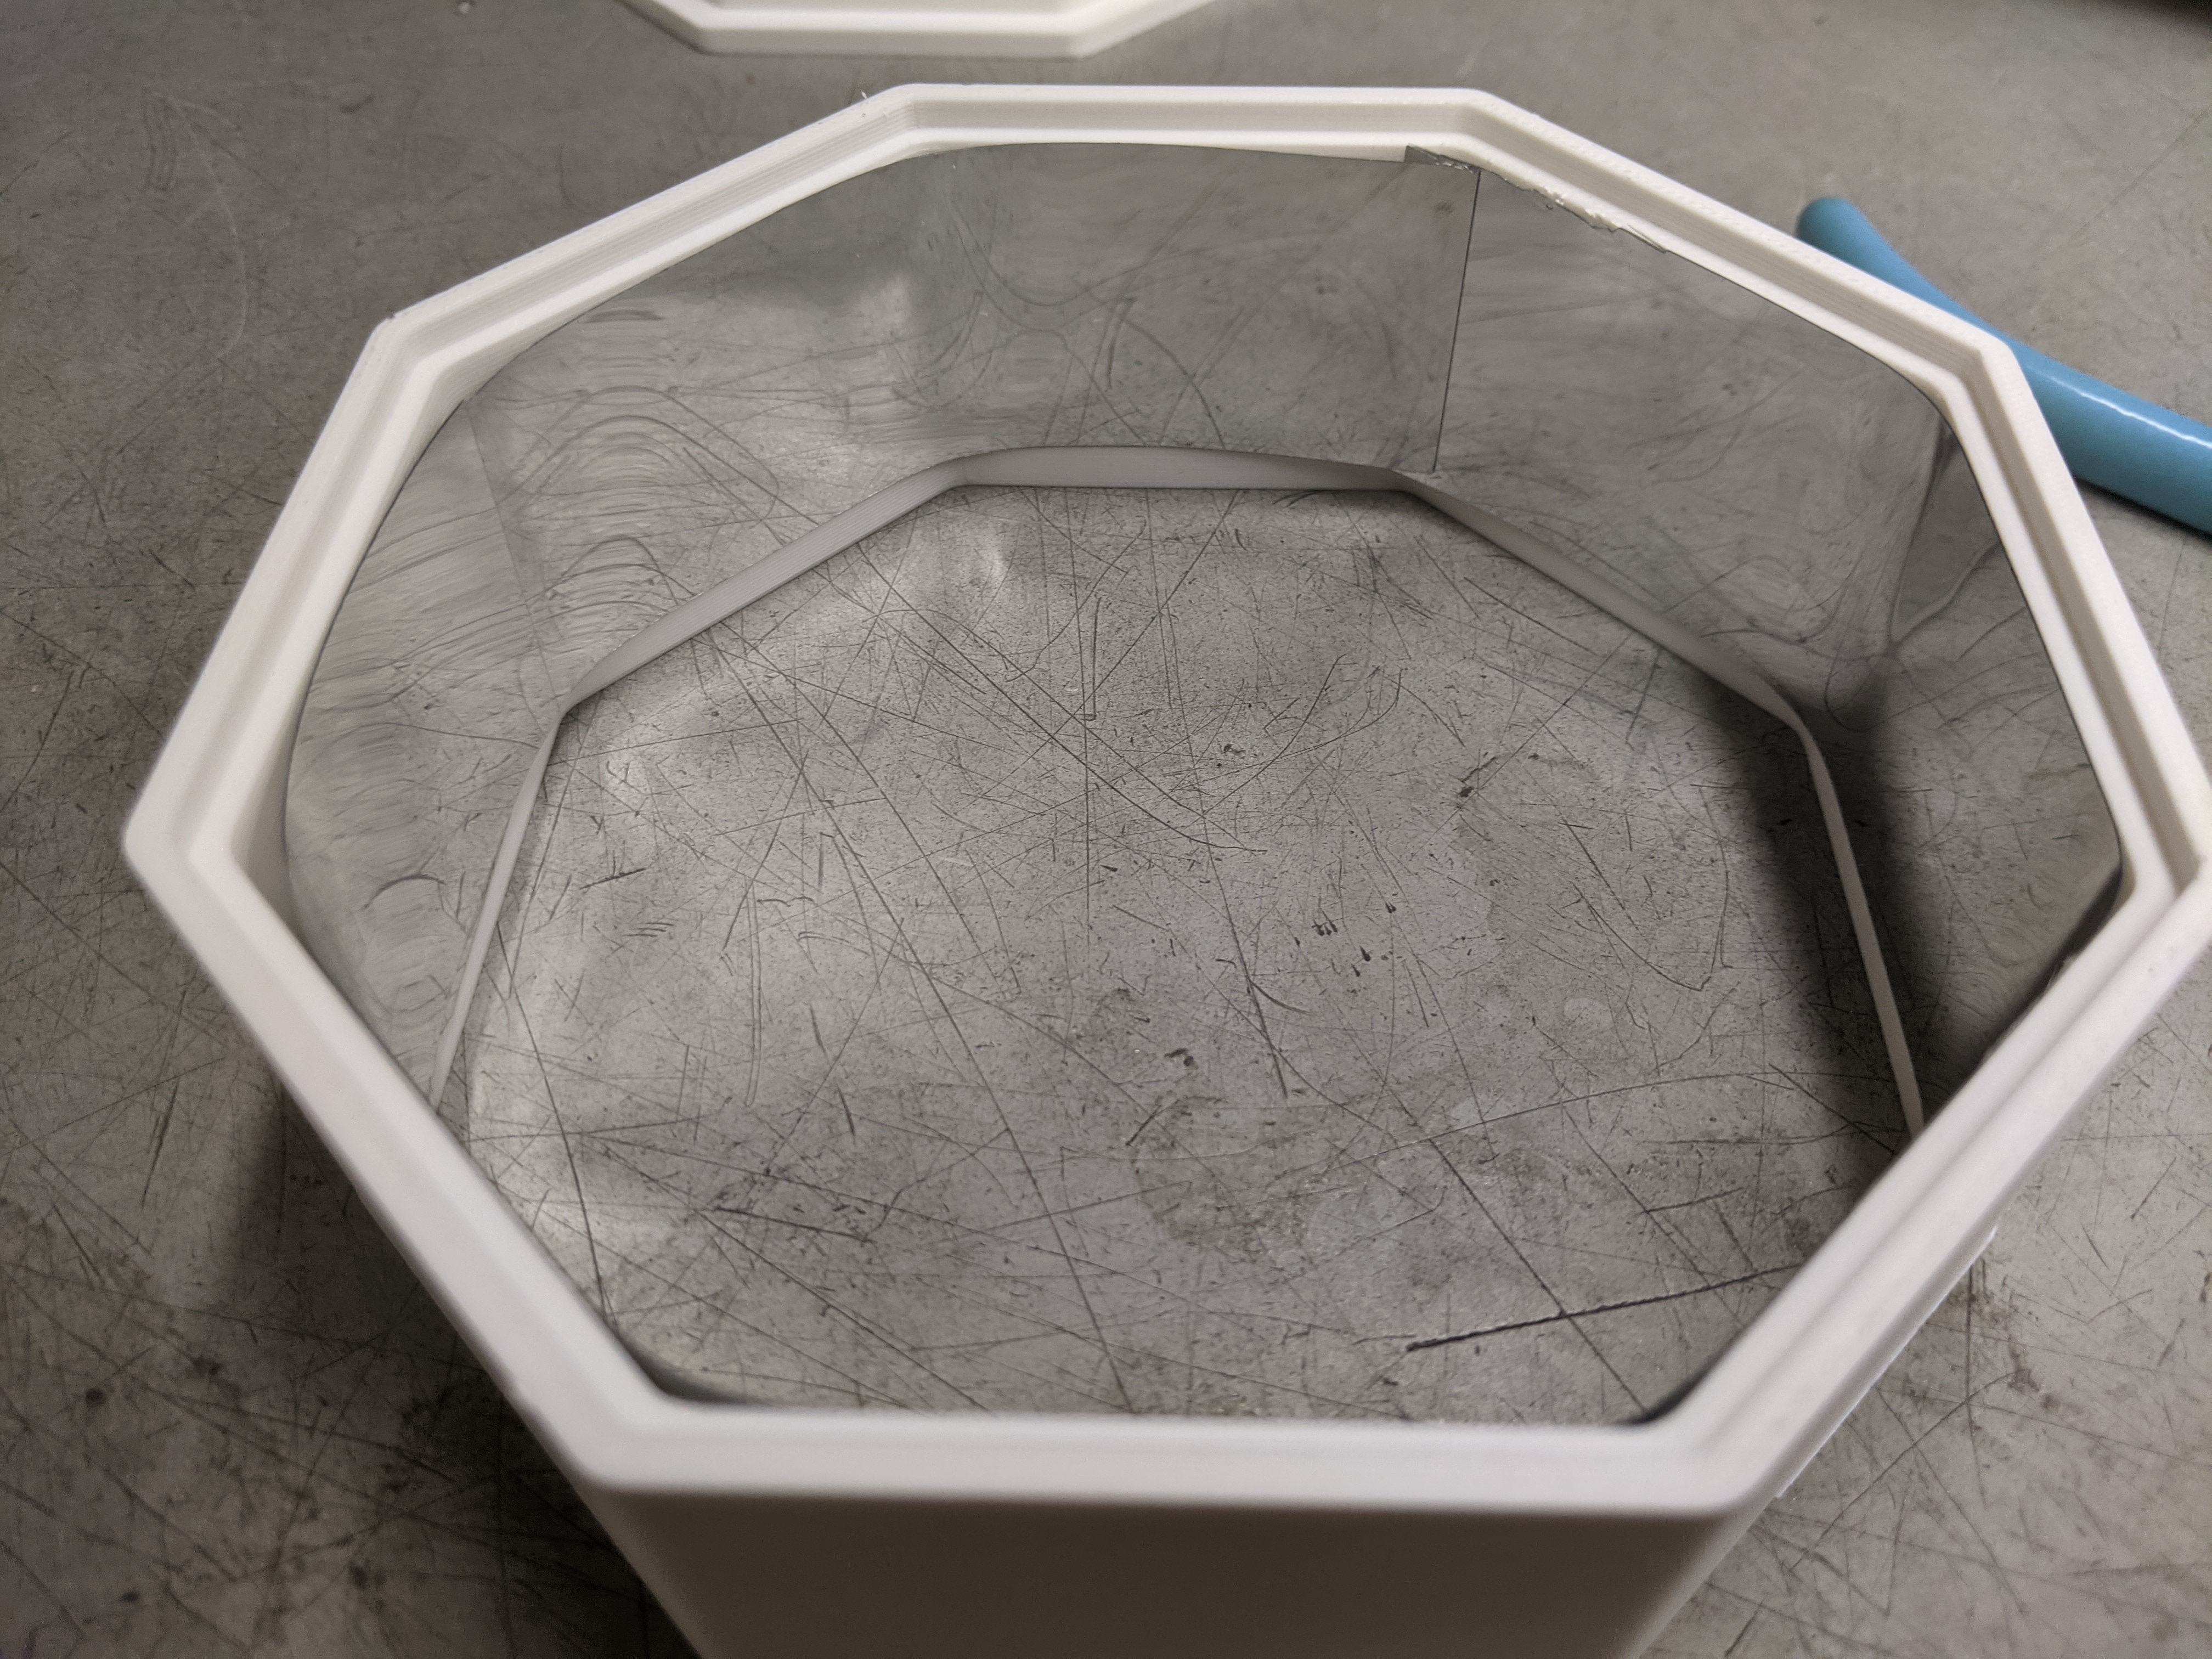
\includegraphics[width=\textwidth/2]{"./reflector.jpg"}
\end{center}

TODO: part number


\end{document}
